\newpage 
\section{Embedding policy, practice and supports to advance academic and research careers}
\label{sec:academic}



\subsection{Reflecting on recruitment practices in the department}


\instr{

\begin{prompt}
\setlength\tabcolsep{6pt} 
\begin{tabu} to \textwidth {@{} X[9] X X }
     \multirow{2}{=}{Recruitment to academic and research posts in the department adheres to institutional policy on recruitment, which includes gender-balanced panels and training for assessors } 
     & \textbf{Yes} & \textbf{No}  \\
     &  \Square & \XBox  \\[.1in] 

\end{tabu}
\setlength\tabcolsep{0pt} 
\end{prompt}
If you answered `no', please comment.
}

The policies that apply to gender-balanced panels and training for selection committee members for academic posts, do not apply to recruiting researchers.  Table~\ref{tab:committee:gender:balance:research} shows that in the previous 3 years only 19\%, on average,  of recruitment committee members for research positions were female, many were entirely male. To address the training requirements and gender-balanced panels, the school will require all committee members to undergo training, e.g., recruitment and selection training (Action~\ref{action:acad:recruittraining}).


\begin{tabbox}[5cm]{!th}
\caption{Selection committee gender balance research}
\label{tab:committee:gender:balance:research}
\footnotesize 

\sisetup{
    group-digits=all,
    group-minimum-digits=4,
    table-format=2.1,
    mode=text,
    reset-text-series = false, 
    text-series-to-math = true,
    reset-text-family=false, 
    text-family-to-math=true
}
\begin{tabular}{p{4cm}
                S[table-format=2.0\%]
                }
\toprule 
Gender & {\%}\\ 
\midrule 
Male & 78\%\\
\hdashline 
Female & 19\% \\
\hdashline 
Unknown & 3\% \\
\bottomrule 
\end{tabular}
\end{tabbox}

% \begin{SCtable}
% \caption{Committee gender balance research}
% \label{tab:committee:gender:balance:research}
% \footnotesize 
% \sisetup{
%     group-digits=all,
%     group-minimum-digits=4,
%     table-format=2.1,
%     mode=text,
%     reset-text-series = false, 
%     text-series-to-math = true,
%     reset-text-family=false, 
%     text-family-to-math=true
% }
% \begin{tabular}{p{4cm}
%                 S[table-format=2.0\%]
%                 }
% \toprule 
% Gender & {\%}\\ 
% \midrule 
% Male & 78\%\\
% \hdashline 
% Female & 19\% \\
% \hdashline 
% Unknown & 3\% \\
% \bottomrule 
% \end{tabular}
% \end{SCtable}


\begin{actionblock}{\ksspace{}School policy on research recruitment}{acad:recruittraining}
\actrecruitmenttraining
\hfill{
    \hypersetup{hidelinks}
    \hyperlink{c7}{\gotoactionsymbol{}}
}
\end{actionblock}




Table~\ref{tab:selection:acad} shows that recruitment for academic posts;  over 70\% of the selection committees had more than 40\% female representation.

\begin{tabbox}{!th}
\caption{Gender equality and selection committees for academic positions}
\label{tab:selection:acad}
\footnotesize 
\sisetup{
    group-digits=all,
    group-minimum-digits=4,
    group-separator = {,},
    table-format=4.1,
    mode=text,
    reset-text-series = false, 
    text-series-to-math = true,
    reset-text-family = false, 
    text-family-to-math = true
}
\begin{tabular}{p{2cm}
                p{9.4cm}
                R{0.7cm}
                R{0.7cm}
                !{\qquad}
                S[table-format=2.0\%]
                }
\toprule
    {Year} & 
    {Competition} & 
    \multicolumn{3}{c}{{\makecell{Selection Committee}}} \\
    \cmidrule{3-5}
    & & {F} & {M} & {\%F}\\
\midrule

2017/18 & Professor of Computer Science & 3 & 5 & 38\% \\ 
\cdashline{2-5}
& Lecturer in Computer Science & 3 & 3 & 50\% \\
\cdashline{2-5}
& Lecturer in Computer Science & 3 & 3 & 50\% \\
\hdashline
2018/19 & Lecturer in Computer Science (x2) & 2 & 4 & 33\% \\
\cdashline{2-5}
& Lecturer in Computer Science (BA Psychology) & 3 & 2 & 60\%\\
\cdashline{2-5}
& Lecturer in Computer Science (BA Digital Humanities) & 3 & 2 & 60\% \\
\cdashline{2-5}
& Lecturer in Computer Science & 2 & 3 & 40\% \\
\midrule
Total & & 19 & 22 & 46\% \\
\bottomrule

\end{tabular}
{
\\[2mm]
\sffamily Note: No recruitment in 2019/2020.
}
\end{tabbox}






\subsection{Provide three years of data on application, shortlist, and appointment rates for recruitment by gender and grade. Where data suggests opportunity for improvement, comment and reflect. Include any other relevant information relating to recruitment processes and practice for academic and research posts in the department. }

Academic recruitment is centrally managed by \ac{HR}. There were nine academic appointments from 2017 to 2019 (Table~\ref{tab:equality:recruitment:academic}).

There were significantly fewer female applicants, particularly for the Professorship in 2017/18. 
No female applicant was appointed in 2017/18, however, in 2018/19,  3 of the 5 appointees were female. 



\begin{tabbox}{!th}
\caption{Gender equality and academic recruitment}
\label{tab:equality:recruitment:academic}
\footnotesize 

\begin{tabular}{P{1.5cm}P{4.6cm}C{1.0cm}
                                C{0.9cm}
                                R{0.7cm}
                                p{0.2cm}
                                C{1.0cm}
                                C{0.9cm}
                                R{0.7cm}
                                p{0.2cm}
                                C{1.0cm}
                                C{0.9cm}
                                R{0.7cm}}
\toprule
    {Year} & 
    {Competition} & 
    \multicolumn{3}{c}{{\makecell{Applicants}}} && 
    \multicolumn{3}{c}{{\makecell{Shortlisted}}} &&
    \multicolumn{3}{c}{{\makecell{Appointed}}}\\
    \cmidrule(l){3-5}\cmidrule(l){7-9}\cmidrule(l){11-13} 
    & & {F} & {M} & {\%F} && {F} & {M} & {\%F} && {F} & {M} & {\%F}\\
\midrule

2017/18 & Professor of Computer Science & 2 & 25 & 7\% && 0 & 7 & 0\% && 0 & 2 & 0\%\\ 
\cdashline{2-13}
& Lecturer in Computer Science & 7 & 15 & 32\% && 4 & 3 & 57\% && 0 & 1 & 0\%\\
\cdashline{2-13}
& Lecturer in Computer Science & 4 & 24 & 14\% && 0 & 7 & 0\% && 0 & 1 & 0\%\\
\hdashline
2018/19 & Lecturer in Computer Science (x2) & 9 & 44 & 17\% && 2 & 7 & 22\% && 1 & 1 & 50\%\\
\cdashline{2-13}
& Lecturer in Computer Science (BA Psychology) & 7 & 12 & 37\% && 3 & 3 & 50\% && 1 & 0 & 100\%\\
\cdashline{2-13}
& Lecturer in Computer Science (BA Digital Humanities) & 8 & 17 & 32\% && 2 & 4 & 33\% && 1 & 0 & 100\%\\
\cdashline{2-13}
& Lecturer in Computer Science & 0 & 6 & 0\% && 0 & 1 & 0\% && 0 & 1 & 0\%\\
\midrule 
Total & & 37 & 143 & 21\% & & 11 & 32 & 26\% && 3 & 6 & 33\% \\
\bottomrule
\end{tabular}
{
\\[2mm]
\sffamily Note: No recruitment in 2019/2020.
}
\end{tabbox}



The school is committed to addressing the gender imbalance across academic staff (Table~\ref{tab:acresstaff}), in particular at \ac{SL} level and above.
It took part in the \ac{SALI} Chair initiative in 2019 and in 2020 for establishing a female professorship for the school. Unfortunately, the school's bid was unsuccessful. In 2021, the school advertised a Professorship in Human Centred Computing. Of the five shortlisted applicants, two were women and both were deemed appointable. Both declined; one citing the high teaching workload as unattractive (Action~\ref{action:acad:transparentworkload}).

While exploring how to increase the number of female applicants for academic posts, it was suggested that the language used in advertisements might be inadvertantly discouraging such applicants:

\begin{myquote}
``... can write a job advert in a way that discourages women from applying – it's the language you use ...''
\end{myquote}

Consequently, the school will adopt gender neutral language and seek to use gender decoders when creating advertisements for academic and research positions (Action~\ref{action:acad:marketing}). Furthermore,  we will actively target female applicants for all posts (Action~\ref{action:acad:femaleonly}).


\begin{actionblock}{\ksspace{}Improve advertising text}{acad:marketing}
\actimproveadvertisingtext
\hfill{
    \hypersetup{hidelinks}
    \hyperlink{c2}{\gotoactionsymbol{}}
}
\end{actionblock}


\begin{actionblock}{\ksspace{}Target suitable female academics and researchers}{acad:femaleonly}
\acttargetfemales
\hfill{
    \hypersetup{hidelinks}
    \hyperlink{c1}{\gotoactionsymbol{}}
}
\end{actionblock}

In the period from 2017 to 2020, 21\% of research appointments in CSIT were female. This is similar to the proportion of female PhD holders in Computer Science, globally. 

The survey revealed that researchers remained unconvinced of adequate training and mentoring opportunities towards promotion (Figure~\ref{fig:research:access}); for researchers, promotion implies either a higher researcher grade (e.g. Senior Research Fellow), or a permanent academic position.

\begin{figbox}{!t}
\caption{Access to training and mentoring needed for promotion (Researchers)}
\label{fig:research:access}
\footnotesize 
    \begin{tabular}{P{5.6cm}p{8cm}}
    \addlinespace 
    I have access to the training and mentoring I need to help me meet the criteria for promotion or to improve my success at promotion & 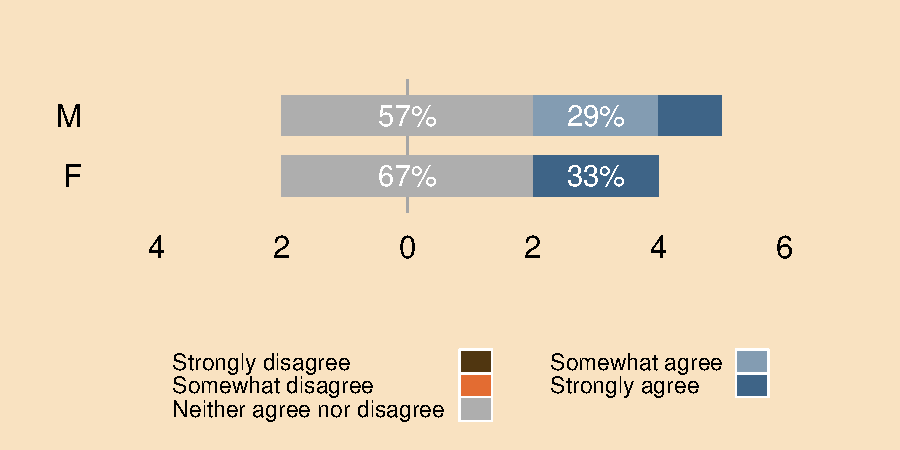
\includegraphics[align=t,trim={0 20mm 15mm 16mm},clip,width=8cm]{fig/careerdev/dirk_accessR.pdf}\\
    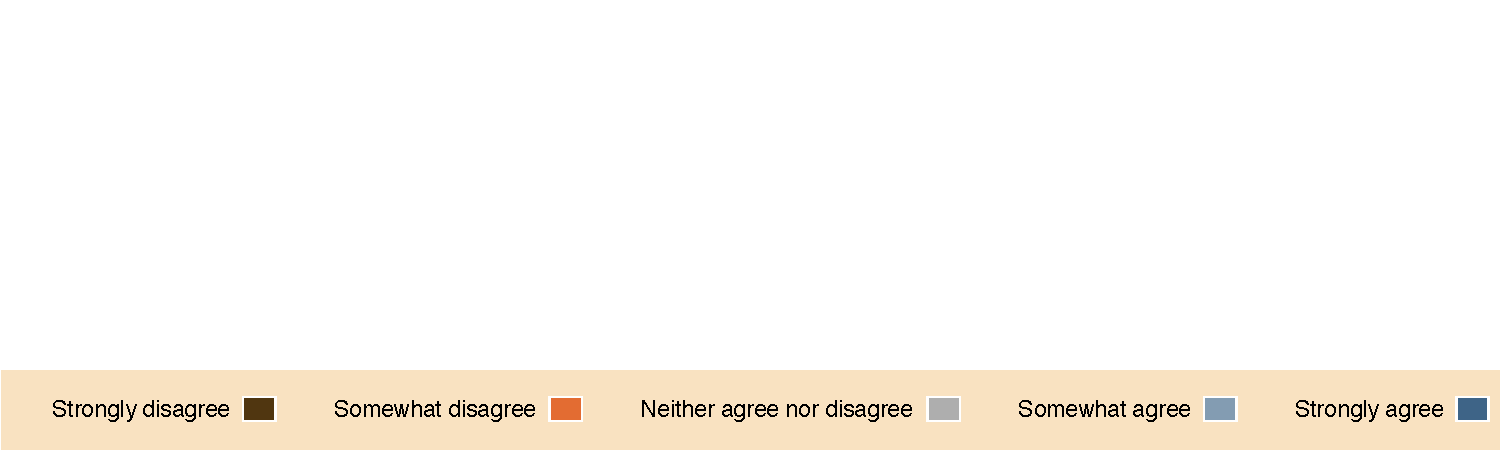
\includegraphics[trim={6mm 0 0 0},clip,width=14.5cm]{fig/legend5col.pdf}
    \end{tabular}
\end{figbox}




In the focus group, researchers requested help be made available with personal development plans (Action~\ref{action:acad:mentorresearchers}).



\begin{actionblock}{\ksspace{}Support researchers with personal development plan}{acad:mentorresearchers}
\actmentorresearchers
\hfill{
    \hypersetup{hidelinks}
    \hyperlink{c4}{\gotoactionsymbol{}}
}
\end{actionblock}

The staff focus group highlighted the need to allow applicants to account for gaps in their CVs --- particularly related to maternity leave and caring responsibilities. 

\begin{myquote}
``There isn’t a guideline, ... that says, look if you have had a family break of any kind, … you have this opportunity to describe it … so that if you have gaps in your CV, you can explain them, because gaps in a CV are a red flag if they're not explained.''
\end{myquote}


Consequently, the school will accept `Leave Statements' as part of its recruitment process (Action~\ref{action:acad:cvgaps}).


\begin{actionblock}{\ksspace{}Consider leave statements}{acad:cvgaps}
\actincludeleavestatement 
\hfill{
    \hypersetup{hidelinks}
    \hyperlink{c6}{\gotoactionsymbol{}}
}
\end{actionblock}


\subsection{Reflecting on academic promotion in your institution, answer the following: }

\instr{
\begin{prompt}
\setlength\tabcolsep{6pt} 
\begin{tabu} to \textwidth {@{} X[8] X X X }
     \multirow{2}{=}{Academic promotion processes, including eligibility criteria, are managed centrally by the institution} & \textbf{Yes} & \textbf{No}  & \textbf{N/A}\\
     &  \XBox & \Square  & \Square \\ 
\end{tabu}
\setlength\tabcolsep{0pt} 
\end{prompt}
}

\instr{If you answered ‘no’, please comment on the department’s role in academic promotions processes. If you answered ‘not applicable’, as prescribed promotion pathways are not in place in your institution, provide comment and reflection on alternative routes for academic career progression.}

\subsection{Provide three years of data on application and success rates for promotion by gender and grade and present results from staff consultation by gender. Where data suggests opportunity for improvement, comment and reflect}

As discussed on Page~\pageref{slboundary}, only one call for promotion (2018/19) was issued from 2017 to 2019, resulting in no successful candidates (Table~\ref{tab:promotion2sl}). 


\begin{tabbox}{!h}
\caption[Promotion applications and outcome to Senior Lecturer]{Promotion applications and outcome to Senior Lecturer (2017-2020)}
\label{tab:promotion2sl}
\footnotesize 

    
\begin{tabular}{p{4cm}                
                C{1cm}
                C{1cm}
                p{0.5cm}
                C{1cm}
                C{1cm}
                p{0.5cm}
                C{1cm}
                C{1cm}}
    
\toprule 
& \multicolumn{2}{c}{Applicants} && \multicolumn{2}{c}{Successful} && \multicolumn{2}{c}{Success rates}\\
\cmidrule{2-3}\cmidrule{5-6}\cmidrule{8-9}
Year  & F & M & & F & M && F & M\\
\midrule
2018/2019 & 0 & 2 & & 0 & 0 && 0\% & 0\% \\        
\bottomrule      

\end{tabular}
{
\sffamily 
\\[.1in]
UCC had no promotion schemes to SL, to Professor (Scale 2) or Progression across the Merit Bar from 2016-2020.
}
\end{tabbox}



Both the staff survey and focus groups revealed that staff are unhappy with the lack of promotion opportunities. 
Many respondents felt that the promotion process and criteria are neither transparent nor fair.  

\begin{figbox}{!ht}
\caption{Access to training and mentoring needed for promotion (Academics)}
\label{fig:academic:access}
\footnotesize
    \begin{tabular}{P{5.6cm}p{8cm}}
    \addlinespace 
    I have access to the training and mentoring I need to help me meet the criteria for promotion or to improve my success at promotion & 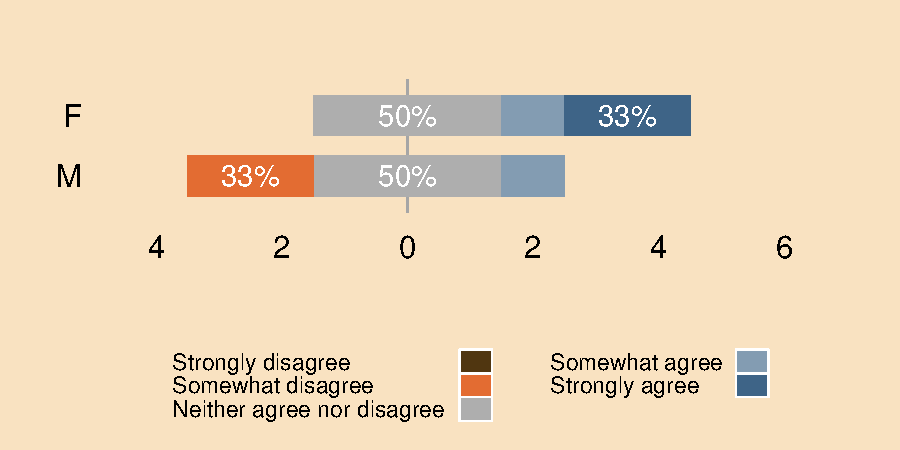
\includegraphics[align=t,trim={0 20mm 15mm 16mm},clip,width=8cm]{fig/careerdev/dirk_accessA.pdf}\\
    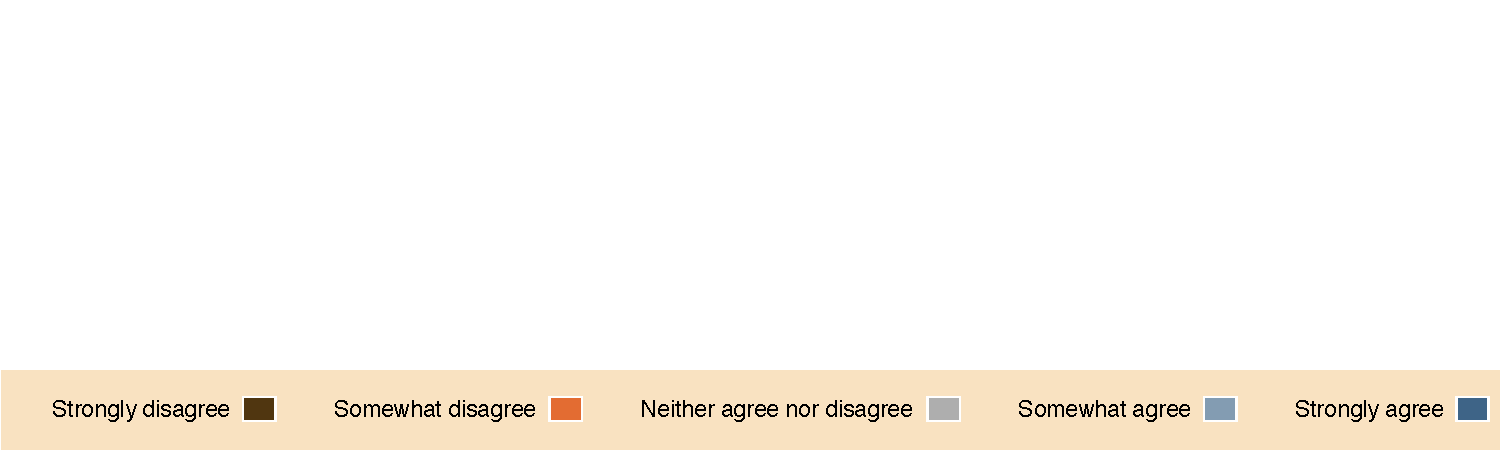
\includegraphics[trim={6mm 0 0 0},clip,width=14.5cm]{fig/legend5col.pdf}\\
    \end{tabular}
\end{figbox}



\begin{myquote}
``There is no promotion scheme... It seems to be an impossible process to ... become a professor in UCC. I’ve kind of given up hope, to be honest.''
\end{myquote}

\begin{myquote}
``In essence, there is no realistic prospect of promotion whatsoever... ''
\end{myquote}


\begin{myquote}
``I don’t think I’ll ever get a [more senior] position, ... I’m never going to get one of those because they do not align with my area of expertise.''
\end{myquote}

Since the consultation, academic progression and promotion schemes underwent a review in 2022. A call for progression across the merit bar opened in 2022. Calls for promotion to SL will open in early 2023 and to Professor (Scale 2) in 2024.

It was decided that a mentoring scheme to support colleagues seeking promotion would benefit all staff and would encourage female staff, in particular, to engage with the system (Action~\ref{action:acad:mentoring}). 



\begin{actionblock}{\ksspace{}Academic mentoring scheme}{acad:mentoring}
\actmentorpromotion
\hfill{
    \hypersetup{hidelinks}
    \hyperlink{c10}{\gotoactionsymbol{}}
}
\end{actionblock}




%

\begin{tabbox}{!th}
\caption{Gender equality and academic recruitment}
\label{tab:equality:recruitment:academic}
\footnotesize 

\begin{tabular}{P{1.5cm}P{4.6cm}C{1.0cm}
                                C{0.9cm}
                                R{0.7cm}
                                p{0.2cm}
                                C{1.0cm}
                                C{0.9cm}
                                R{0.7cm}
                                p{0.2cm}
                                C{1.0cm}
                                C{0.9cm}
                                R{0.7cm}}
\toprule
    {Year} & 
    {Competition} & 
    \multicolumn{3}{c}{{\makecell{Applicants}}} && 
    \multicolumn{3}{c}{{\makecell{Shortlisted}}} &&
    \multicolumn{3}{c}{{\makecell{Appointed}}}\\
    \cmidrule(l){3-5}\cmidrule(l){7-9}\cmidrule(l){11-13} 
    & & {F} & {M} & {\%F} && {F} & {M} & {\%F} && {F} & {M} & {\%F}\\
\midrule

2017/18 & Professor of Computer Science & 2 & 25 & 7\% && 0 & 7 & 0\% && 0 & 2 & 0\%\\ 
\cdashline{2-13}
& Lecturer in Computer Science & 7 & 15 & 32\% && 4 & 3 & 57\% && 0 & 1 & 0\%\\
\cdashline{2-13}
& Lecturer in Computer Science & 4 & 24 & 14\% && 0 & 7 & 0\% && 0 & 1 & 0\%\\
\hdashline
2018/19 & Lecturer in Computer Science (x2) & 9 & 44 & 17\% && 2 & 7 & 22\% && 1 & 1 & 50\%\\
\cdashline{2-13}
& Lecturer in Computer Science (BA Psychology) & 7 & 12 & 37\% && 3 & 3 & 50\% && 1 & 0 & 100\%\\
\cdashline{2-13}
& Lecturer in Computer Science (BA Digital Humanities) & 8 & 17 & 32\% && 2 & 4 & 33\% && 1 & 0 & 100\%\\
\cdashline{2-13}
& Lecturer in Computer Science & 0 & 6 & 0\% && 0 & 1 & 0\% && 0 & 1 & 0\%\\
\midrule 
Total & & 37 & 143 & 21\% & & 11 & 32 & 26\% && 3 & 6 & 33\% \\
\bottomrule
\end{tabular}
{
\\[2mm]
\sffamily Note: No recruitment in 2019/2020.
}
\end{tabbox}




\subsection{Reflecting on opportunities for staff development reviews, answer the following:}\label{sec:2e}

\instr{
\begin{prompt}
\setlength\tabcolsep{6pt} 
\begin{tabu} to \textwidth {@{} X[8] X X @{}}
     \multirow{2}{=}{The institution operates a development review process, or equivalent, for academic and research staff} & \textbf{Yes} & \textbf{No}  \\
     &  \XBox & \Square   \\ 
\end{tabu}
\setlength\tabcolsep{0pt} 
\end{prompt}
}

\instr{
If you answered ‘yes’, comment and reflect on the implementation of this institution-level process in the department. This should include: 
\begin{itemize}
\item	data on uptake by gender;
\item	results from staff consultation presented by gender;
\item	information on any additional department-level opportunities for staff to discuss professional development. 
\end{itemize}

\noindent If you answered ‘no’, provide detail on department-level opportunities for staff to discuss professional development, including data on uptake by gender and results from staff consultation presented by gender. 
}\label{acad:pdrs}



UCC operates a Performance Development and Review System (\ac{PDRS}), which applies to all staff, except for those with less than 50\% FTE, less than a year left on a contract, staff on probation, on long term sick leave, or within two years of retirement. As part of the process, staff can discuss their development needs with their line manager. The process did not operate from 2017 to 2020; it was scheduled to restart in 2019, but this was further postponed due to Covid-19 restrictions in 2019 and 2020. 


\begin{figbox}[10cm]{!b}
    \caption{Awareness of the Performance Development Review System}
     %trim={<left> <lower> <right> <upper>}
    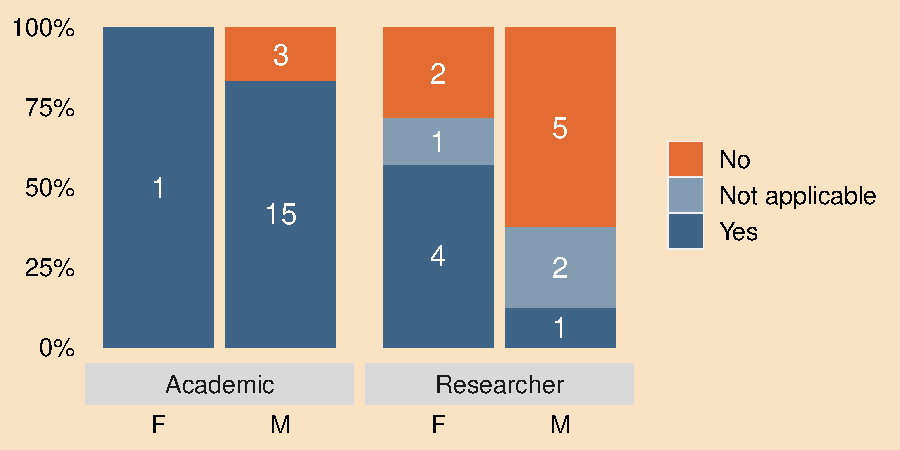
\includegraphics[trim={0 0 0 0},clip,width=9cm]{fig/awareness.pdf}
    \label{fig:awareness}
\end{figbox}


The staff survey revealed that the majority of academic staff were aware of the PDRS process (100\% female, 80\% male). 
However, the majority of research staff were unaware of the process (Figure~\ref{fig:awareness}). 
The survey data suggests that the female academic staff respondent was satisfied with the opportunity to engage with the 
\ac{HOS} on performance and development, approximately 15\% of male academic staff are not satisfied (neutral to or disagree with) with those opportunities (Figure~\ref{fig:acadcareerdev}). 



\begin{figbox}{!t}
    \sffamily 
    \footnotesize 
    \raggedright 
    \caption{Academic career development opportunities}        
    
    \begin{tabular}{P{5cm}p{9cm}}
    \addlinespace 
    
    I am satisfied with the opportunities I have to discuss my career progress with my line-manager &
    % left down right up
    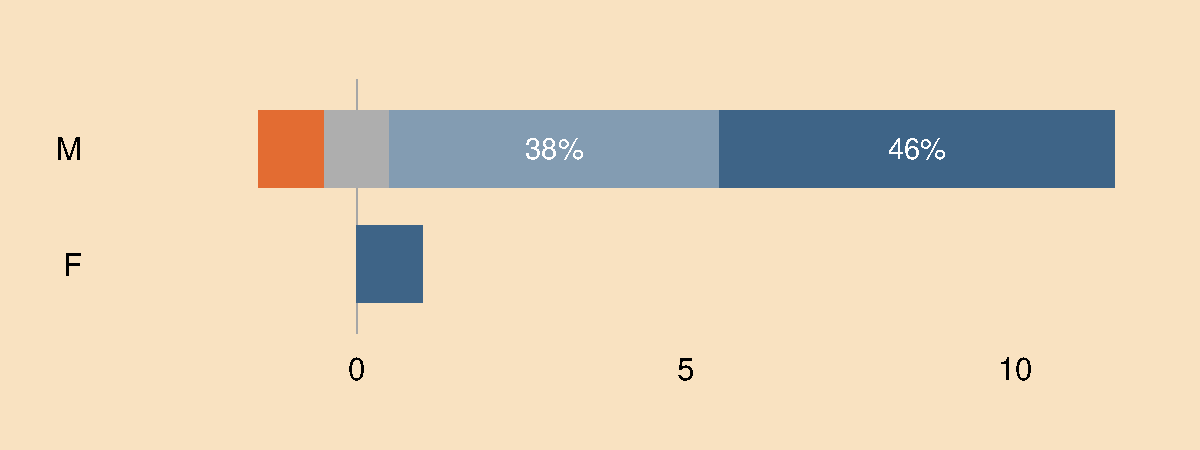
\includegraphics[align=t,trim={0 4mm 10mm 17mm} ,clip,width=9cm]{fig/careerdev/dirk_career.pdf}\\

\hdashline

    I am satisfied with the opportunities I have to discuss promotion opportunities with my line-manager
    &
    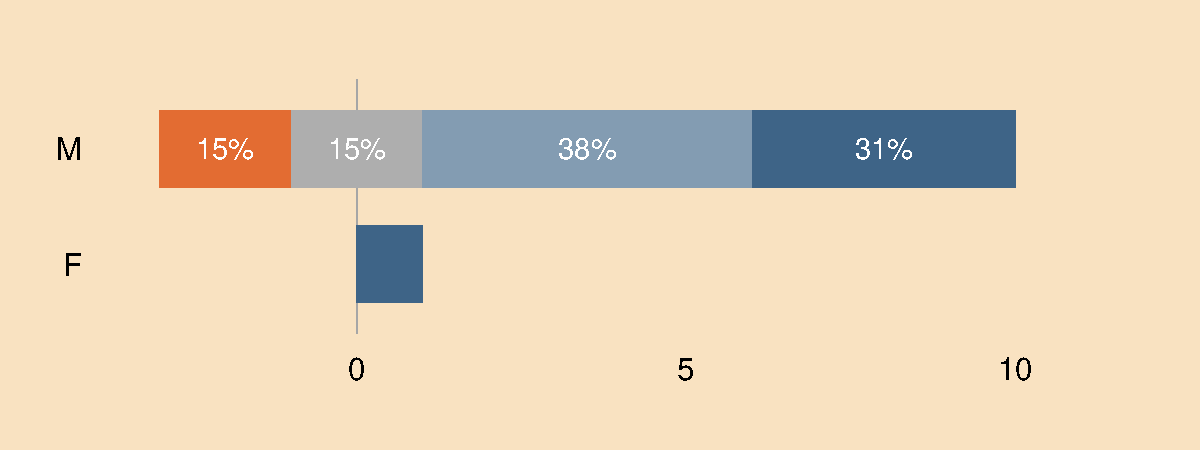
\includegraphics[align=t,trim={0 4mm 10mm 17mm} ,clip,width=9cm]{fig/careerdev/dirk_promotion.pdf}\\
   
\hdashline

    I am satisfied with the opportunities I have to discuss my work-load with my line manager
    &
    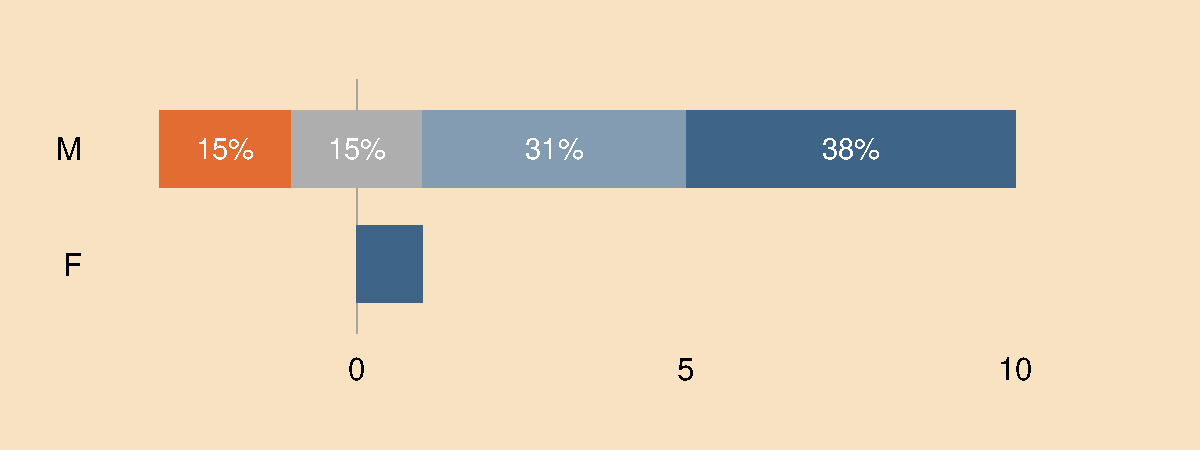
\includegraphics[align=t,trim={0 4mm 10mm 17mm} ,clip,width=9cm]{fig/careerdev/dirk_workload.pdf}\\

\hdashline

    I am satisfied with the opportunities I have to discuss my work objectives with my line manager
    &
    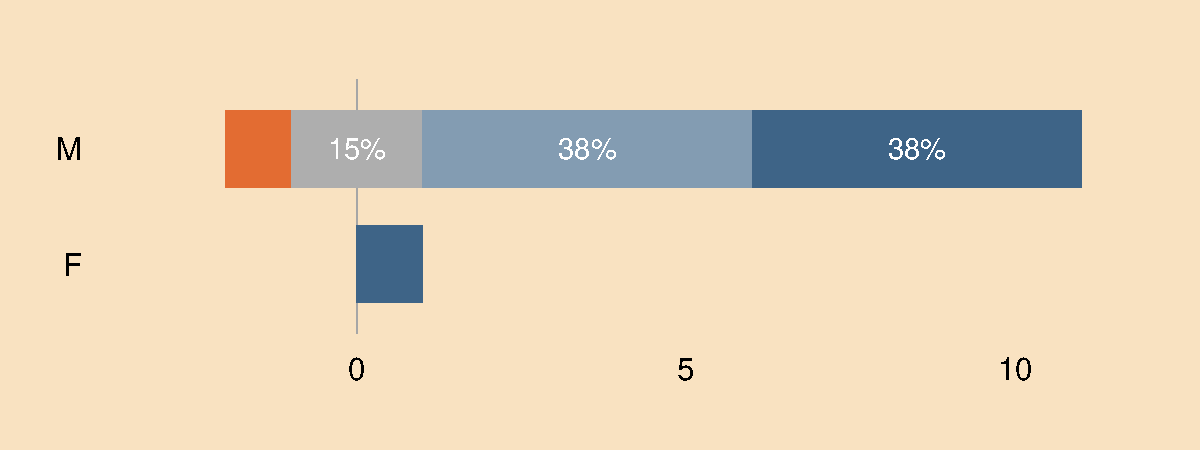
\includegraphics[align=t,trim={0 4mm 10mm 17mm} ,clip,width=9cm]{fig/careerdev/dirk_objectives.pdf}\\

    %% Legend
    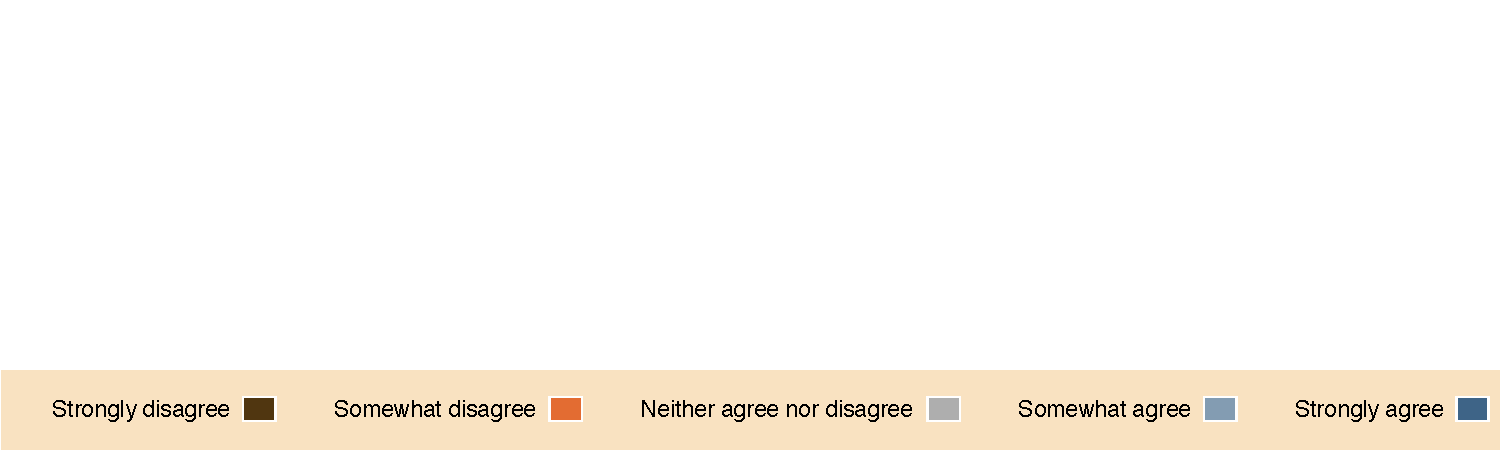
\includegraphics[trim={6mm 0 0 0},clip,width=14.5cm]{fig/legend5col.pdf}\\

    \end{tabular}
    \label{fig:acadcareerdev}
\end{figbox}


\pagebreak
Comments on the \ac{PDRS} process during the academic staff focus group were mixed:

\begin{myquote}
``The only conversations that I have with a line manager or head of department would be [about teaching schedules] ...''
\end{myquote}

\begin{myquote}
`` ... he was very helpful. He tried to map out where are your weaknesses? [and supported me to develop in those areas]''
\end{myquote}



It is hoped that Action~\ref{action:acad:pdrs} would address these concerns.
% Figure with awareness of PDRS process.


\begin{actionblock}{\ksspace{}Restart PDRS process}{acad:pdrs}
\actrestartpdrs
\hfill{
    \hypersetup{hidelinks}
    \hyperlink{c13}{\gotoactionsymbol{}}
}
\end{actionblock}

Researcher feedback from the staff survey and focus groups was mixed (Figure~\ref{fig:research:career:planning}). The survey data indicated that approximately 70\% of respondents never had a `development needs' meeting with their line manager (PI). Approximately 90\%  have no personal development plan, 90\% have no training objectives and 67\% of those who do, consider that they are not meeting their training objectives.
Nevertheless, respondents commended the development opportunities available within UCC and felt supported by the school to avail of those opportunities (Figure~\ref{fig:research:career:development}). 


  
\begin{figbox}{!hb}
    \caption{Support for researcher career planning}
    \label{fig:research:career:planning}

    \sffamily 
    \footnotesize 
    \raggedright 
    \begin{tabular}{P{5cm}!
                    {\quad}
                    p{9cm}}
    \addlinespace
    I am satisfied with the opportunities I have to discuss career progress with my PI & 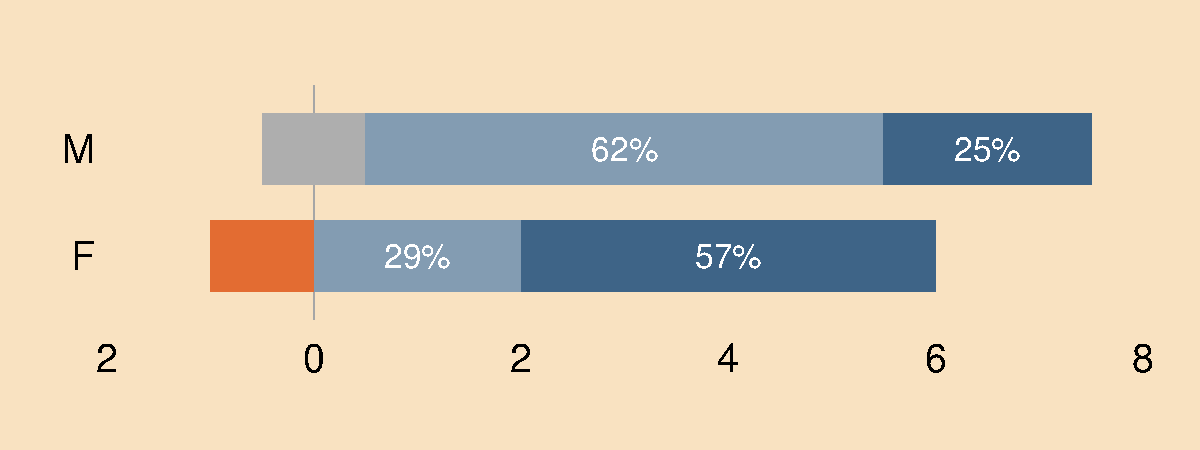
\includegraphics[align=t,trim={0 4mm 7mm 17mm},clip,width=8cm]{fig/careerplan/dirk_carprogress.pdf}\\

\hdashline
    I am satisfied with the opportunities I have to discuss promotion opportunities with my PI & 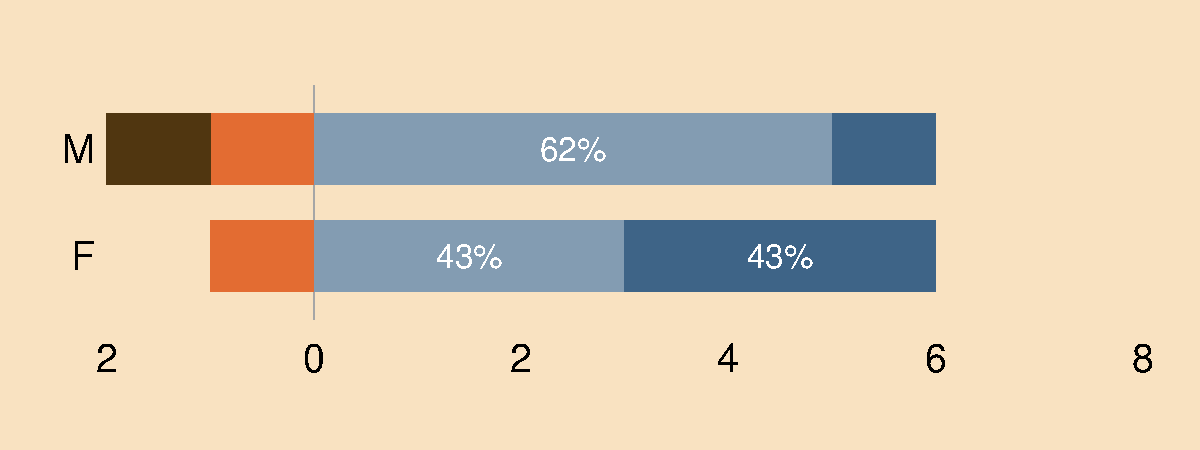
\includegraphics[align=t, trim={0 4mm 7mm 17mm}, clip, width=8cm]{fig/careerplan/dirk_carpromotion.pdf}\\
\hdashline
    I discuss training and mentoring opportunities with my PI &
    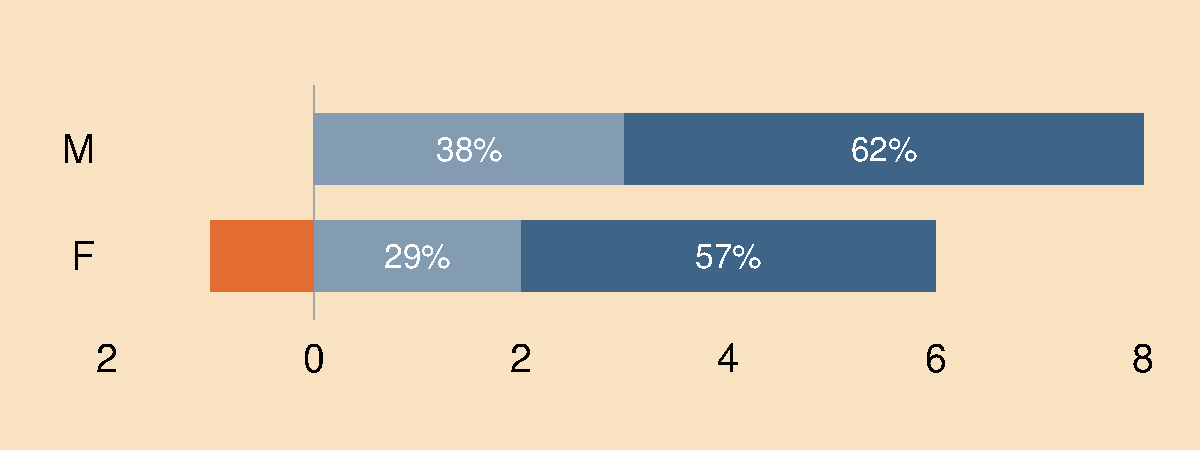
\includegraphics[align=t, trim={0 4mm 7mm 17mm}, clip, width=8cm]{fig/careerplan/dirk_carmentoring.pdf}\\

    %% Legend.
    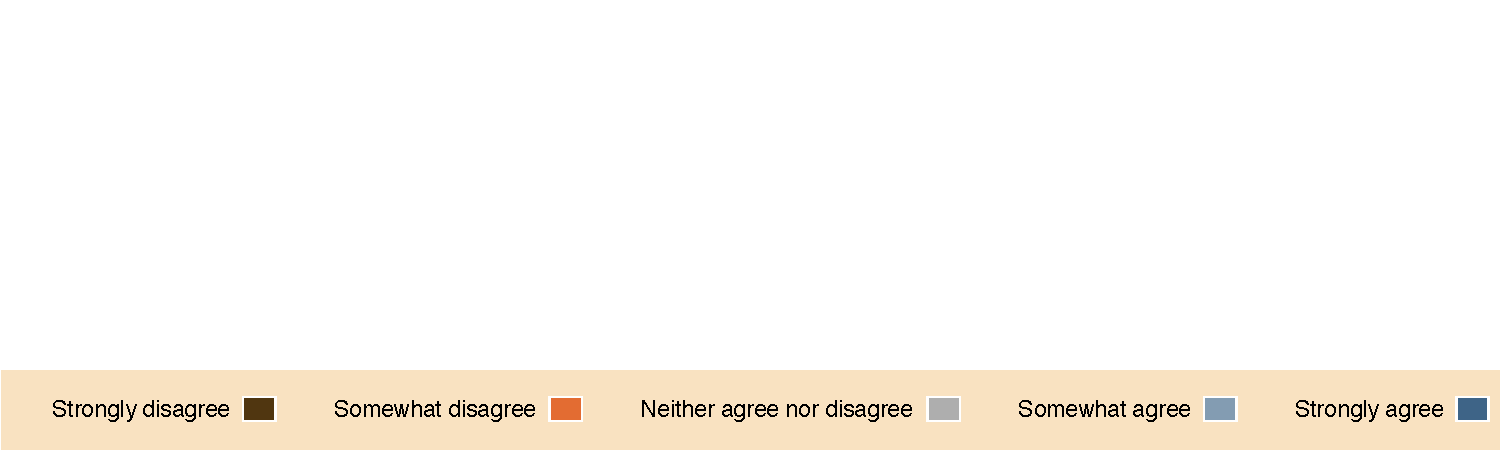
\includegraphics[trim={6mm 0 0 0},clip,width=14.5cm]{fig/legend5col.pdf}\\
    
    \end{tabular}        
\end{figbox}


Overall, evidence suggests that many academic and research staff are unhappy with career development opportunities and supports (Action~\ref{action:acad:pdrs}). 


\begin{figbox}{!t}
    \caption{Research staff career development}
    \label{fig:research:career:development}
     %trim={<left> <lower> <right> <upper>}

    \sffamily
    \raggedright
    \footnotesize
    \begin{tabular}{P{5.5cm}p{8cm}}
    \addlinespace
    Have you met with your PI to prepare a Professional Development Plan?  & 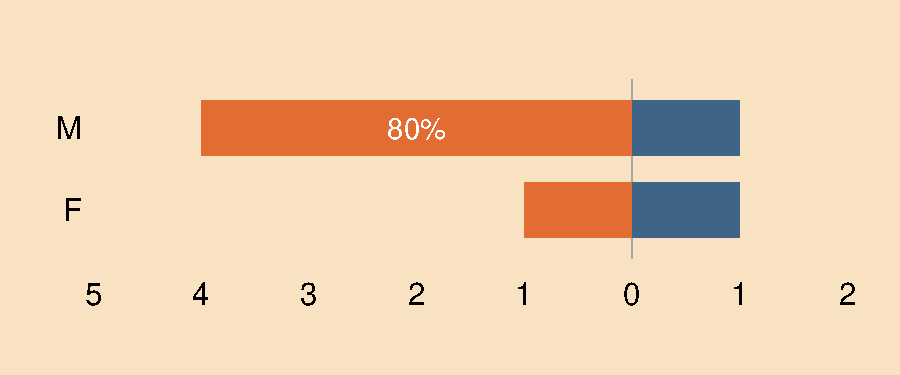
\includegraphics[align=t,trim={0 0 0 16mm},clip,width=8cm]{fig/rescareerdev/dirk_havemet.pdf}\\
\hdashline
    Do you have a current professional development plan? & 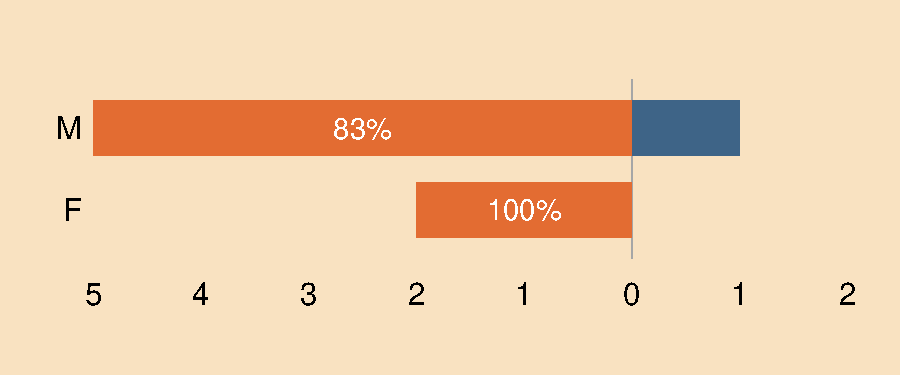
\includegraphics[align=t,trim={0 0 0 16mm},clip,width=8cm]{fig/rescareerdev/dirk_haveplan.pdf}\\
\hdashline
    Does your Professional Development Plan identify specific training objectives? & 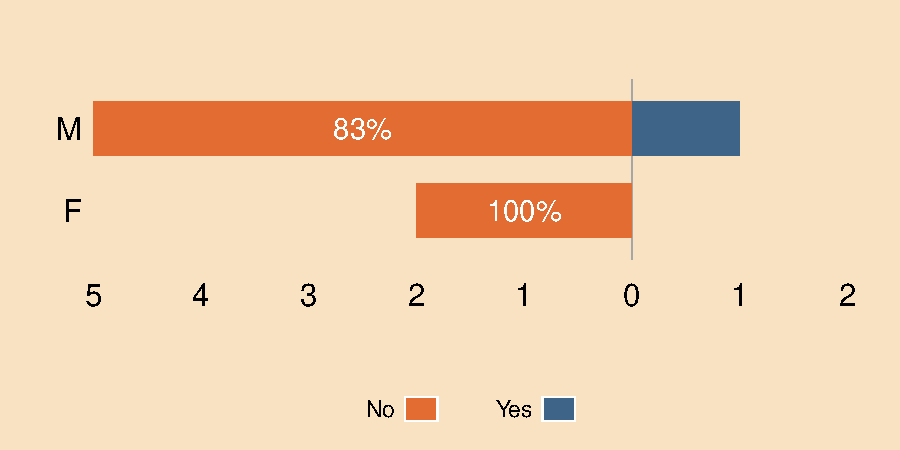
\includegraphics[align=t,trim={0 0 0 16mm},clip,width=8cm]{fig/rescareerdev/dirk_specify.pdf}\\
    
    \end{tabular}
    
\end{figbox}




\subsection{Comment and reflect on department engagement with institution-level supports for academic and research staff career progression as well as any department-level support available. This should include results from staff consultation presented by gender and may include, but is not limited to, support given to staff to:}\label{sec:2f}
\instr{
\begin{itemize}
\item	apply for research funding;
\item	develop excellence in teaching and learning.
\end{itemize}
}

\subsubsection{Comments and Reflections on Institution-level Supports for Career Progression} 

UCC provides training and development programmes for academic and research staff. These include personal and professional development, management and leadership development, and staff wellbeing, which are coordinated by HR, the \ac{OVPRI}, and the Office of the VP for Teaching and Learning. 
Table~\ref{tab:training:academic} 
shows the uptake of development opportunities by academic staff in the report period.  


\begin{tabbox}{!th}
    \footnotesize 
    \caption{Training uptake by academic staff by gender}
    \label{tab:training:academic}
    %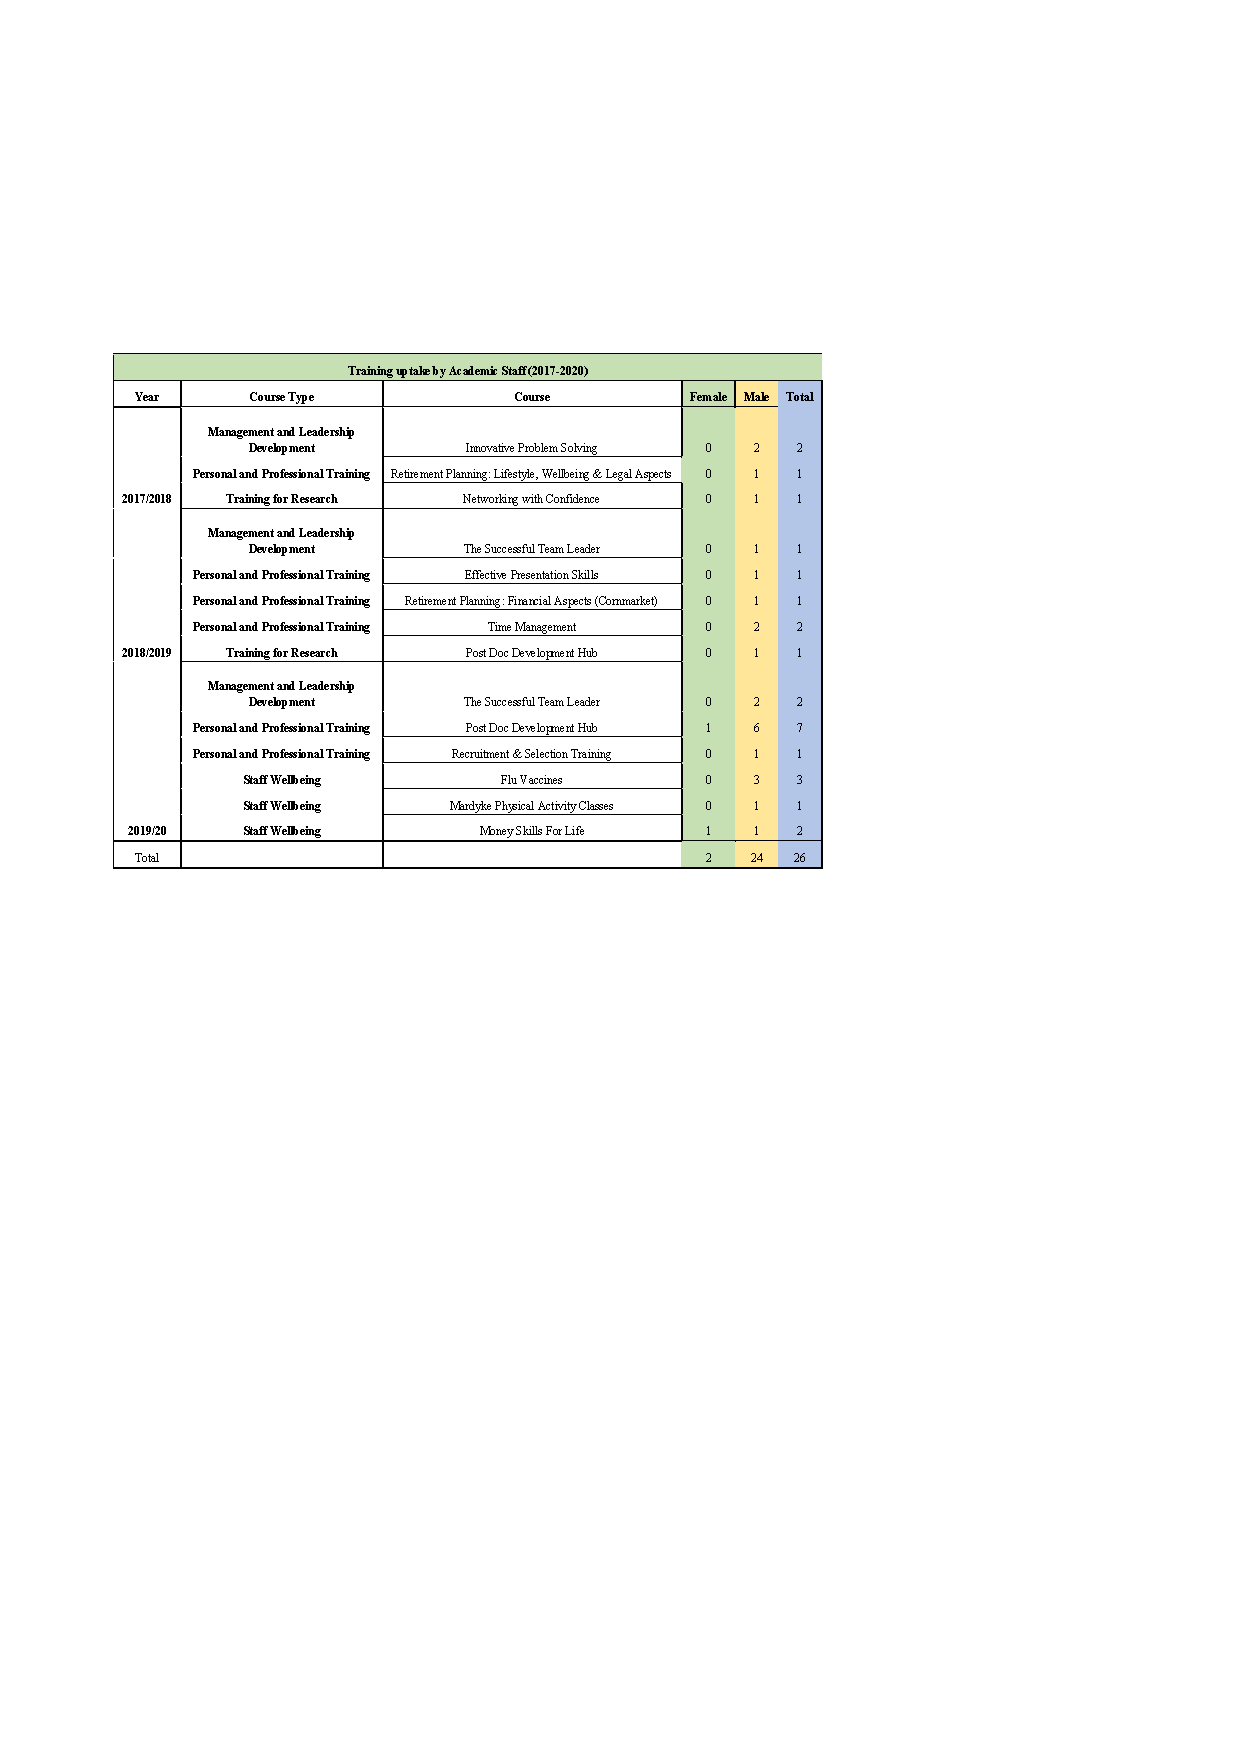
\includegraphics[width=\textwidth]{fig/table4.pdf}
    
    \begin{tabular}{p{2cm}
                    p{9.5cm}
                    !{\qquad}
                    R{1cm}
                    R{1cm}}
    
    \toprule 
    Year & Course & F & M \\
    \midrule
    
    2017/18 &  Innovative Problem Solving & 0 & 2\\
    \cdashline{2-4}
    & Retirement Planning: Lifestyle, wellbeing, and legal aspects & 0 & 1\\
    \cdashline{2-4}
    &  Networking with Confidence & 0 & 1\\
    \hdashline
    2018/19 &  The Successful Team Leader & 0 & 1\\
    \cdashline{2-4}
    & Effective Presentation Skills & 0 & 1 \\
    \cdashline{2-4}
    & Retirement Planning: Financial Aspects & 0 & 1 \\
    \cdashline{2-4}
    & Time Management & 0 & 2 \\
    \cdashline{2-4}
    & Post Doc Development Hub & 0 & 1 \\
    \hdashline
    2019/20 & The Successful Team Leader & 0 & 2 \\
    \cdashline{2-4}
    & Post Doc Development Hub  & 1 & 6 \\
    \cdashline{2-4}
    & Recruitment and Selection Training & 0 & 1 \\
    \cdashline{2-4}
    & Flu Vaccines & 0 & 3\\
    \cdashline{2-4}
    & Mardyke Physical Activity Classes  & 0 & 1\\
    \cdashline{2-4}
    & Money Skills for Life & 1 & 1\\
    \midrule 
    Total & & 2 & 24 \\
    
    \bottomrule      
         
    \end{tabular}
\end{tabbox}





Irish universities consider postdoctoral staff as `research trainees.' UCC provides many training and development opportunities via its PostDoc Development Hub.\footnote{\url{https://www.ucc.ie/en/hr/research/devhub/}} 
Table~\ref{tab:training:postdoc} shows these courses and their uptake in the report period. The data do not indicate how many researchers availed of these, but the uptake is limited, particularly among male researchers. 
 

\newpage 
\begingroup
%TC:ignore

\renewcommand\arraystretch{1.4}

\begin{mdframed}[backgroundcolor=orangebg,
                 rightline=false,
                 leftline=false,
                 topline=false,
                 bottomline=false,
                 innertopmargin=0pt,
                 ]
\footnotesize                 
\begin{longtable}{p{2cm}
                p{9.5cm}
                !{\qquad}
                R{1cm}
                R{1cm}}
               
\vspace*{-22pt}
\crule{12mm}{3mm}\\[-7mm]

\caption{Training uptake by research staff, by gender}\label{tab:training:postdoc}\\
\toprule
    Year & Course & F & M \\
\midrule
\endfirsthead
%
\endhead
%
\endfoot
\bottomrule 
\endlastfoot
    
    2017/18 & Developing and consolidating your career & 2 & 0\\
    \cdashline{2-4}
    & Project Management Part 1 & 1 & 0 \\
    \cdashline{2-4}
    & Project Management Part 2 & 1 & 0 \\
    \cdashline{2-4}
    & Grant Writing & 1 & 0 \\
    \cdashline{2-4}
    & Leading a Research Team & 1 & 0 \\
    \cdashline{2-4}
    & Research Data Management & 1 & 0 \\
    \hdashline
    2018/19  & Lean Yellow Belt Training & 1 & 1 \\
    \cdashline{2-4}
    & Active Listening Skills & 1 & 0 \\
    \cdashline{2-4}
    & Communicating With Impact - Managers/Team Leaders & 1 & 1 \\
    \cdashline{2-4}
    & Developing Positive and Assertive Communication Skills & 0 & 1 \\
    \cdashline{2-4}
\pagebreak 
\multicolumn{2}{l}{\normalsize \textbf{Table \thefigure{}} Training uptake by research staff, by gender (continued)}\\
\midrule 

    & Engaging People Who Are Anxious, Distressed, Angry & 0 & 2 \\
    \cdashline{2-4}
    & Identifying and Responding To Students In Distress & 0 & 1 \\
    \cdashline{2-4}
    & Managing Stress In The Workplace & 0 & 1 \\
    \cdashline{2-4}
    & The Effective Employee & 0 & 4 \\
    \cdashline{2-4}
    & Time Management & 0 & 2 \\
    \cdashline{2-4}
    & Unconscious Bias Training & 0 & 2 \\
    \cdashline{2-4}
    & Maximising Professional Effectiveness & 1 & 0 \\
    \cdashline{2-4}
    & Grant Writing & 0 & 1 \\
    \cdashline{2-4}
    & Presentation Skills & 1 & 10\\
    \cdashline{2-4}
    & Commercial Awareness and Knowledge Transfer & 0 & 1 \\
    \cdashline{2-4}
    & Data Management & 2 & 0 \\
    \cdashline{2-4}
    & Funding Your Research & 1 & 0 \\
    \cdashline{2-4}
    & Leading a Research Team & 1 & 0 \\
    \cdashline{2-4}
    & Managing Yourself Through Change & 1 & 0 \\
    \cdashline{2-4}
    & Statistics for Researchers & 1 & 0 \\
    \cdashline{2-4}
    & Teaching and Learning & 1 & 0 \\
    \hdashline
    2019/20 & Change Management & 0 & 1 \\
    \cdashline{2-4}
    & Communicating With Impact - Managers/Team Leaders & 1 & 0\\
    \cdashline{2-4}
    & Critical Thinking For Effective Decisions & 0 & 1 \\
    \cdashline{2-4}
    & Engaging People Who Are Anxious, Distressed, Angry & 1 & 0 \\
    \cdashline{2-4}
    & Flu Vaccines & 0 & 3 \\
    \cdashline{2-4}
    & Introduction To Project Management & 1 & 0 \\
    \cdashline{2-4}
    & Money Skills For Life & 1 & 1 \\
    \cdashline{2-4}
    & Networking Using Drama and Improvisation Techniques & 0 & 1 \\
    \cdashline{2-4}
    & Remote Working Workshop - Employee & 1 & 0\\
    \cdashline{2-4}
    & The Successful Team Leader & 0 & 2 \\
    \cdashline{2-4}
    & Time Management & 0 & 1 \\
    \cdashline{2-4}
    & UCC Health and Wellness Workshops & 1 & 0 \\
    \cdashline{2-4}
    & Winning The Stress Game - Stress Management Info Session & 1 & 1 \\
    \cdashline{2-4}
    & Project Management & 2 & 0 \\
    \cdashline{2-4}
    & Statistics for Researchers & 1 & 0 \\
    \cdashline{2-4}
\pagebreak 
\multicolumn{2}{l}{\normalsize \textbf{Table \thefigure{}} Training uptake by research staff, by gender (continued)}\\
\midrule 
    & Funding Your Research & 1 & 0 \\
    \cdashline{2-4}
    & Making That Transition & 1 & 0 \\
    \cdashline{2-4}
    & Presentation Skills for Research Staff & 1 & 1 \\
    \cdashline{2-4}
    & Motivation Skills for Research Staff & 1 & 0 \\
    \cdashline{2-4}
    & Communication Skills for Researchers & 1 & 0 \\
    \midrule 
    Total & & 34 & 29\\
    \bottomrule      
    
\end{longtable}
\end{mdframed}

%TC:endignore
\endgroup 

There was a marked difference between female and male staff taking up training opportunities (Figure~\ref{fig:training}). The female respondant was happy with the training opportunities and their relevance, the male staff were less happy. They had a lack of awareness, relevance and availability of training opportunities, a perceived lack of support by line manager to participate in training, a perceived lack of opportunity to attend conferences, and some reported a lack of opportunity to present their work to school peers.

\begin{figbox}{!h}
    \caption{Training awareness}
    \label{fig:training}
    % left lower right upper
    

    \sffamily
    \raggedright
    \footnotesize
    \begin{tabular}{P{3.5cm}p{10cm}}
    \addlinespace
    
    I am aware of training opportunities available to me (Academics) &   
    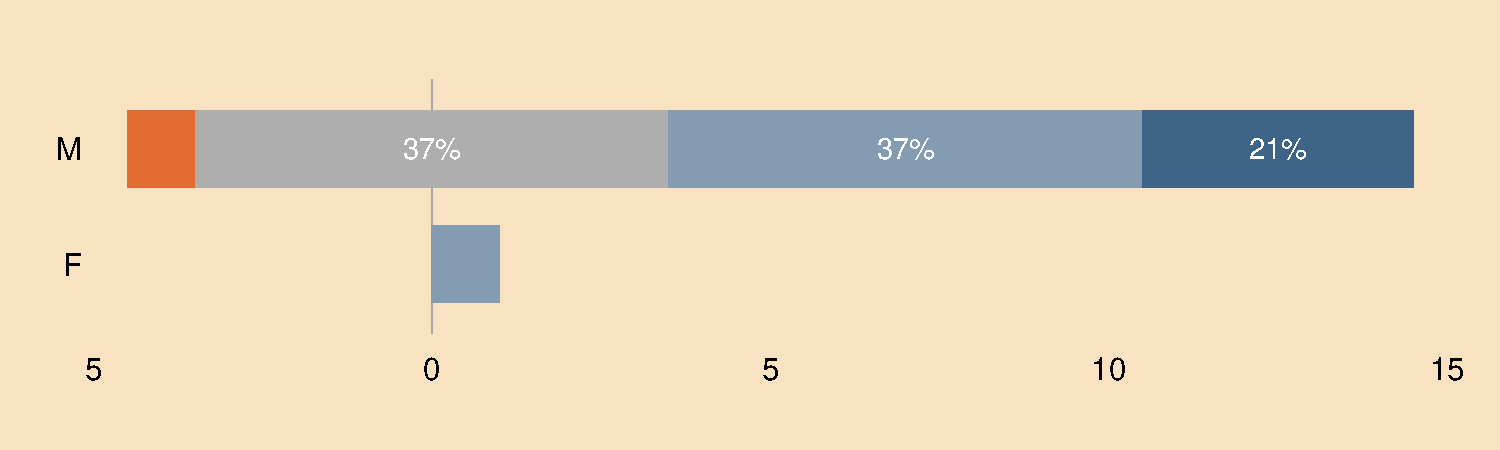
\includegraphics[align=t,trim={0mm 16mm 0 16mm},clip,width=11cm]{fig/training/dirk_trainingV2aA.pdf}\\
    As above, for Researchers & 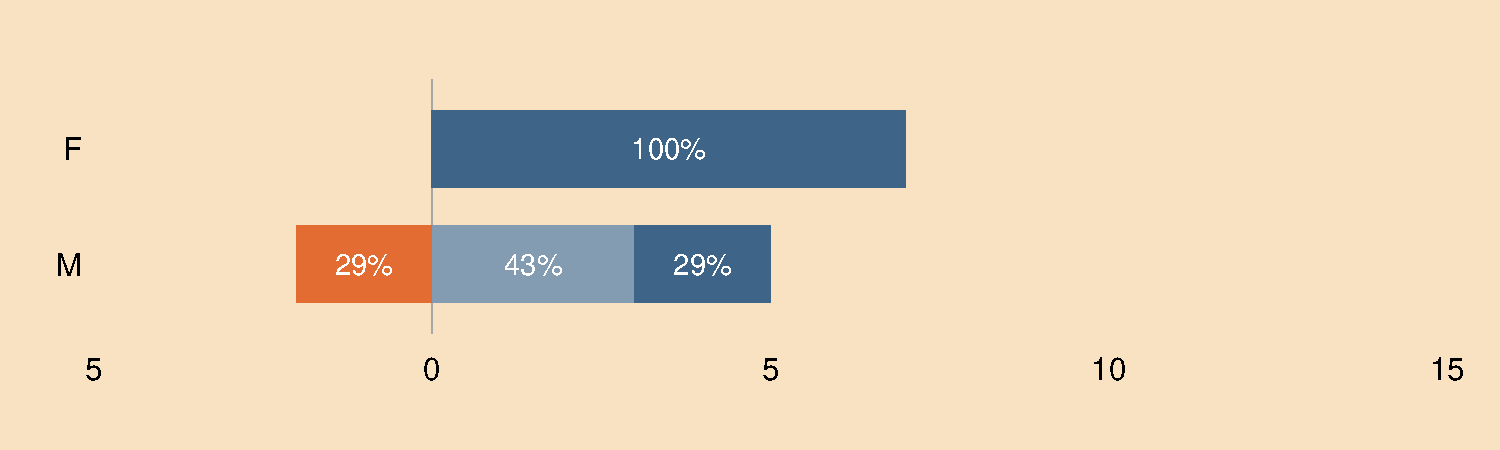
\includegraphics[align=t,trim={0mm 4mm 0 18mm},clip,width=11cm]{fig/training/dirk_trainingV2aR.pdf}\\
    

    \hdashline
    The relevance of the training opportunities is clear to me (Academics) &   
    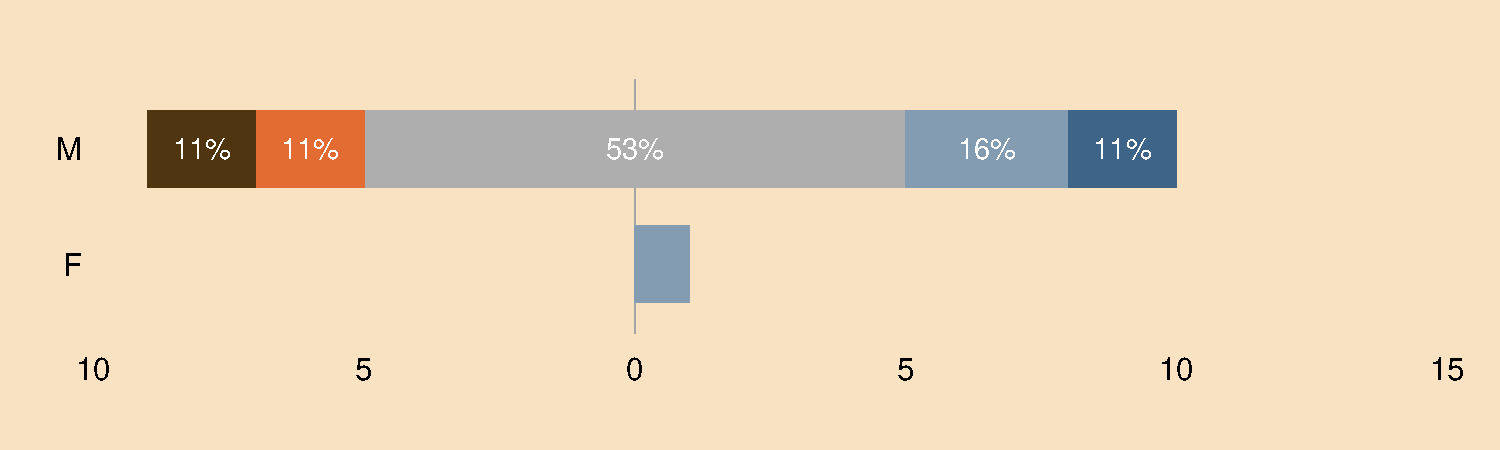
\includegraphics[align=t,trim={0mm 16mm 0 16mm},clip,width=11cm]{fig/training/dirk_trainingV2bA.pdf}\\

    As above, for Researchers &   
    
\includegraphics[align=t,trim={0mm 4mm 0 18mm},clip,width=11cm]{fig/training/dirk_trainingV2bR.pdf}\\
    
    \hdashline
    I am satisfied with the training opportunities available to me (Academics) &   
    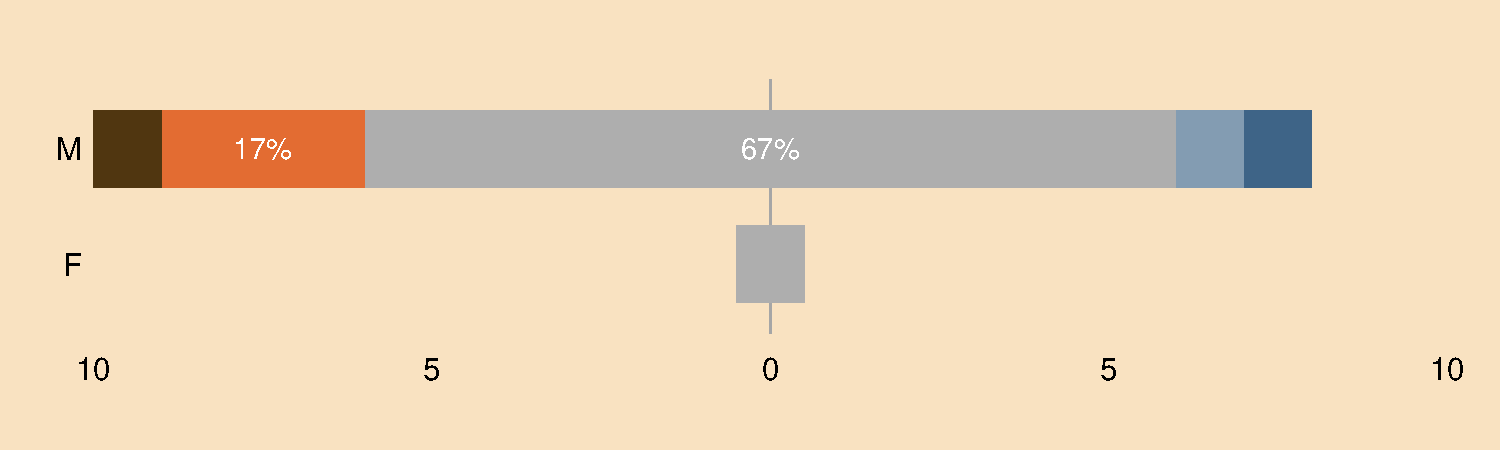
\includegraphics[align=t,trim={0mm 16mm 0 16mm},clip,width=11cm]{fig/training/dirk_trainingV2cA.pdf}\\

    As above, for Researchers &   
    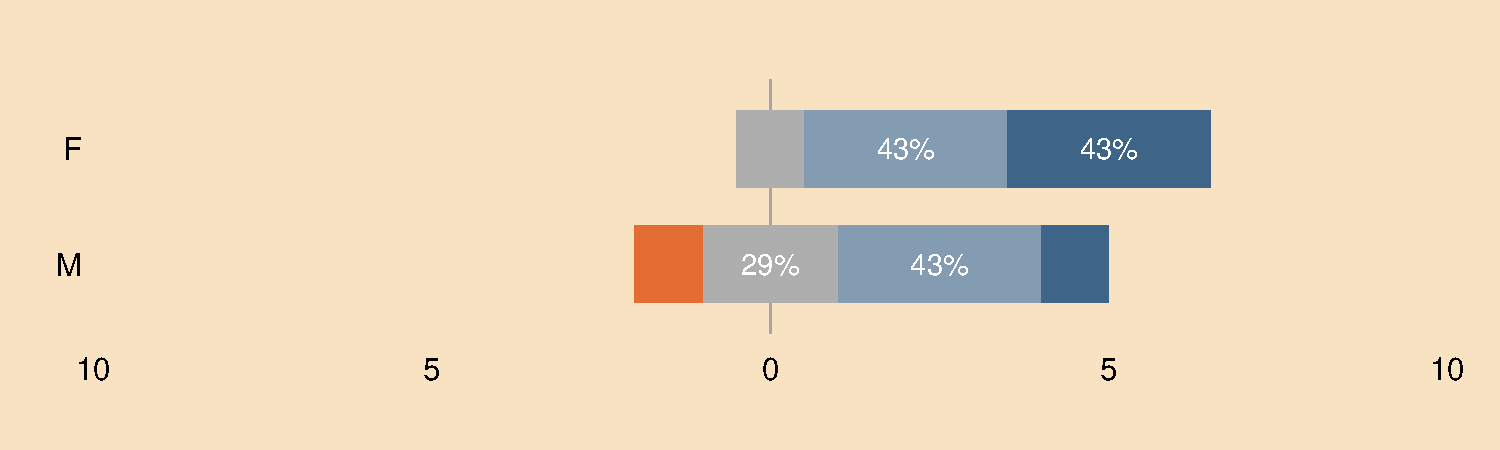
\includegraphics[align=t,trim={0mm 4mm 0 18mm},clip,width=11cm]{fig/training/dirk_trainingV2cR.pdf}\\


    % %% Legend
    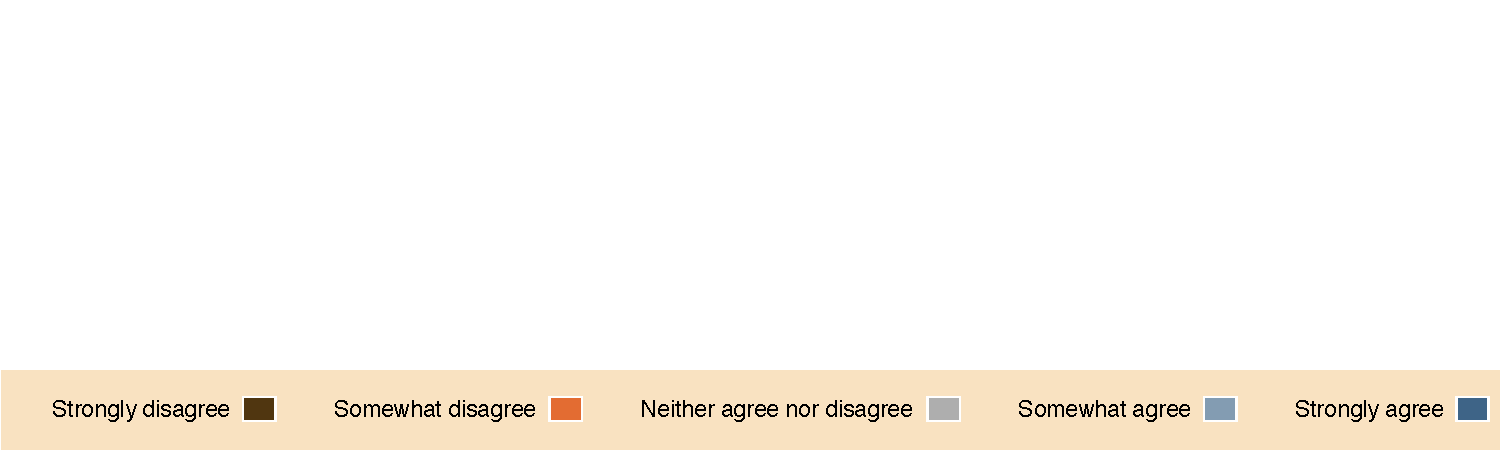
\includegraphics[trim={6mm 0 0 0},clip,width=14.5cm]{fig/legend5col.pdf}\\
    
     \end{tabular}
    
\end{figbox}



Research staff have a more positive view and more balance can be seen between male and female respondents (Figure~\ref{fig:training}). 
A desire was expressed for better communication on training and development opportunities:

\begin{myquote}
``It's important to keep training to keep up to date. I'd like more open discussion around training needs and requirements.''
\end{myquote}

\begin{myquote}
“Unfortunately, I have never heard or seen any email where funding for training has been circulated or promoted.''
\end{myquote}

Academic staff in the focus group were satisified with the school supports and with training offered centrally, but they perceived the uptake to be low. They suggested that the school should echo these opportunities to the staff:

\begin{myquote}
``Those kind of courses [like CIRTL – Centre for Integration of Research, Teaching, and Learning] should be advertised by the department … courses that we can improve … project management skills, soft skills, hard skills … I think that would really benefit us going forward.''
\end{myquote}

Research staff in the focus group would like to see more support for research staff development at school level. Currently, support for career development mainly comes from their respective research centres and groups. 
Consequently, not all researchers may have the same opportunities; researchers who were not part of a centre or large group reported being isolated. As mentioned, the PDRS will restart (Action~\ref{action:acad:pdrs}), which will incorporate career development for research staff, and the PDRS will also serve as a mechanism to make staff aware of training opportunities. 





\subsubsection{Support for Research Funding Applications}

Figure~\ref{fig:fundingsupport} presents results regarding perceived importance, opportunities, and support for research funding, disaggregated by staff category (academic, research) and gender. 
Overall, staff perceived opportunities to apply for research funding is important to their professional development.
The data revealed a number of issues.

%TC:ignore

\begin{mdframed}[backgroundcolor=orangebg,
                 rightline=false,
                 leftline=false,
                 topline=false,
                 bottomline=false,
                 innertopmargin=0pt,
                 ]
\footnotesize                 
\begin{longfigure}{P{4.5cm}p{10cm}}
                    
               
\vspace*{-24pt}
\crule{12mm}{3mm}\\[-7mm]

\caption{Support for funding}
\label{fig:fundingsupport}\\


\endfirsthead
%
\endhead
%
\endfoot
%
\endlastfoot
    
    & \\    
    \multirow{2}{=}{Opportunities to apply for research funding are important for my professional development (Academics) \\[6mm] As above, for researchers} &   
    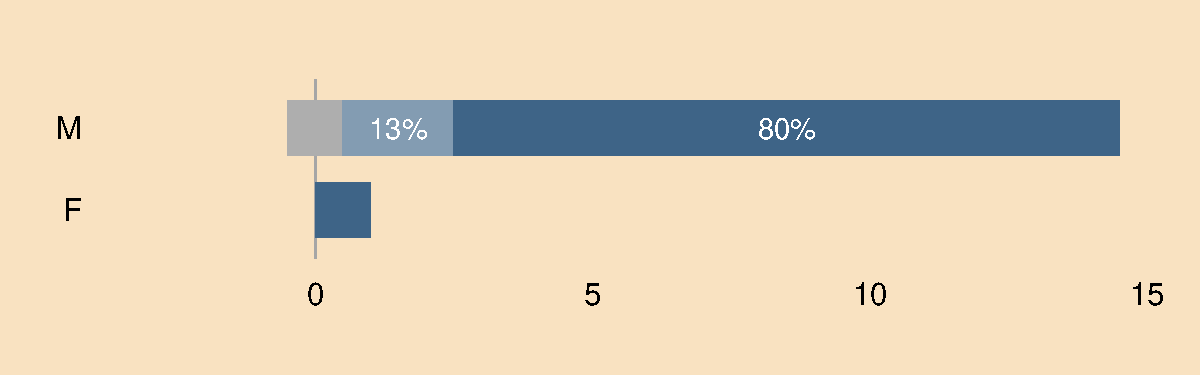
\includegraphics[align=t,trim={0mm 16mm 0 16mm},clip,width=10cm]{fig/support/dirk_supportV2aA.pdf}\\

    &   
    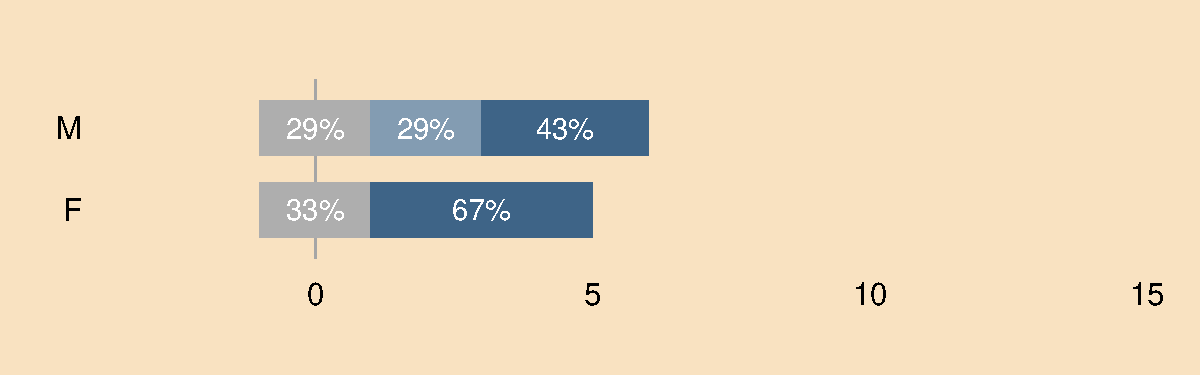
\includegraphics[align=t,trim={0mm 2mm 0 16mm},clip,width=10cm]{fig/support/dirk_supportV2aR.pdf}\\

\hdashline
\addlinespace 
    \multirow{2}{=}{I am satisfied with the opportunities available to me to apply for research funding (Academics) \\[6mm] As above, for researchers}
    &
    
\includegraphics[align=t,trim={0mm 16mm 0 16mm},clip,width=10cm]{fig/support/dirk_supportV2bR.pdf}\\

    &
    
\includegraphics[align=t,trim={0mm 2mm 0 16mm},clip,width=10cm]{fig/support/dirk_supportV2bR.pdf}\\
    
\hdashline    
 \addlinespace    
    \multirow{2}{=}{I am satisfied with the support available within the school to those applying for research funding (Academics) \\[6mm] As above, for researchers} 
    &
    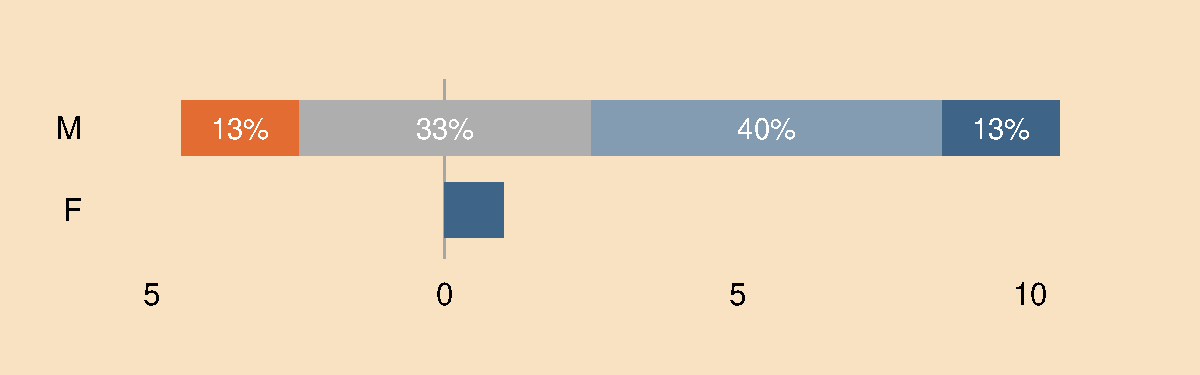
\includegraphics[align=t,trim={0mm 17mm 0 16mm},clip,width=10cm]{fig/support/dirk_supportV2cA.pdf}\\
    
    &
    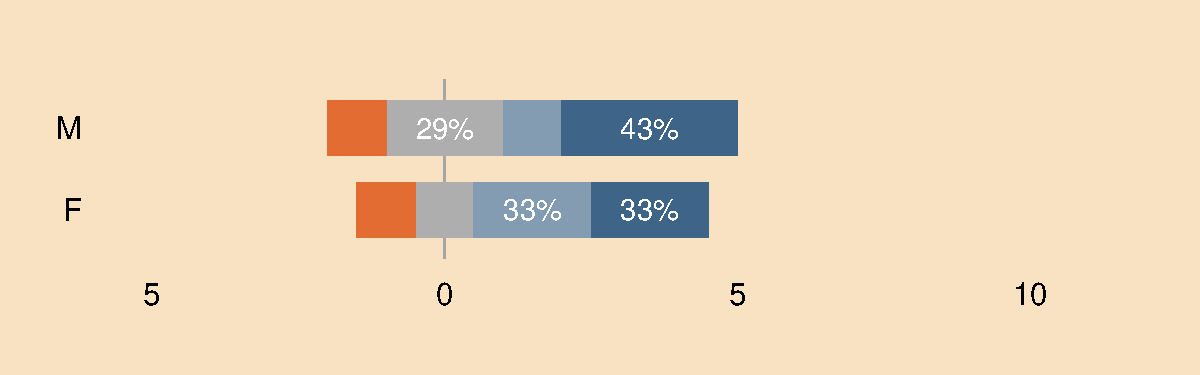
\includegraphics[align=t,trim={0mm 2mm 0 16mm},clip,width=10cm]{fig/support/dirk_supportV2cR.pdf}\\

\hdashline
\pagebreak 

\multicolumn{2}{l}{\normalsize \textbf{Figure \thefigure{}} Support for funding (continued)}\\

\addlinespace 
    \multirow{2}{=}{I am satisfied with the support offered by UCC (e.g. OVPRI, College Research Support Officers) to those applying for research funding (Academics) \\[6mm] As above, for researchers}
    &
    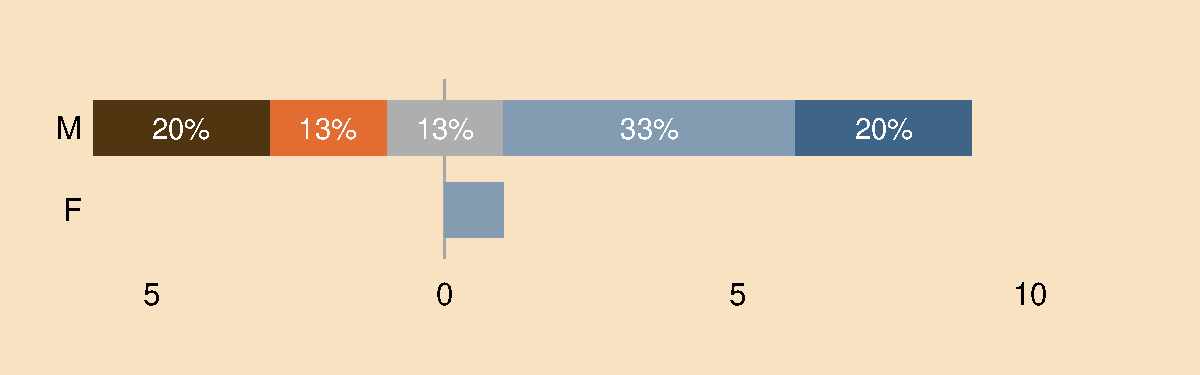
\includegraphics[align=t,trim={0mm 17mm 0 16mm},clip,width=10cm]{fig/support/dirk_supportV2dA.pdf}\\
    
    &
    
\includegraphics[align=t,trim={0mm 2mm 0 16mm},clip,width=10cm]{fig/support/dirk_supportV2dR.pdf}\\

\hdashline 
%\addlinespace 

\addlinespace 
    \multirow{2}{=}{Support is available in my school for applicants whose funding applications are unsuccessful \\[6mm] As above, for researchers}
    &
    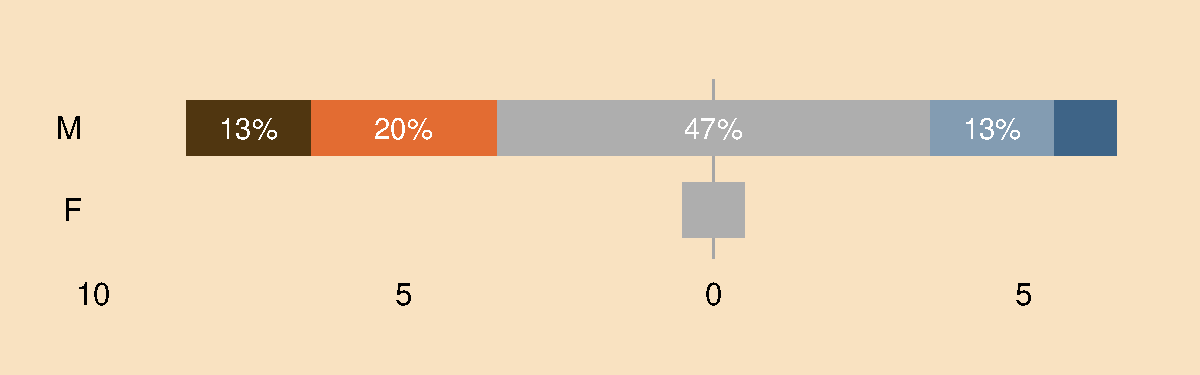
\includegraphics[align=t,trim={0mm 20mm 0 16mm},clip,width=10cm]{fig/support/dirk_supportV2eA.pdf}\\
    
    &
    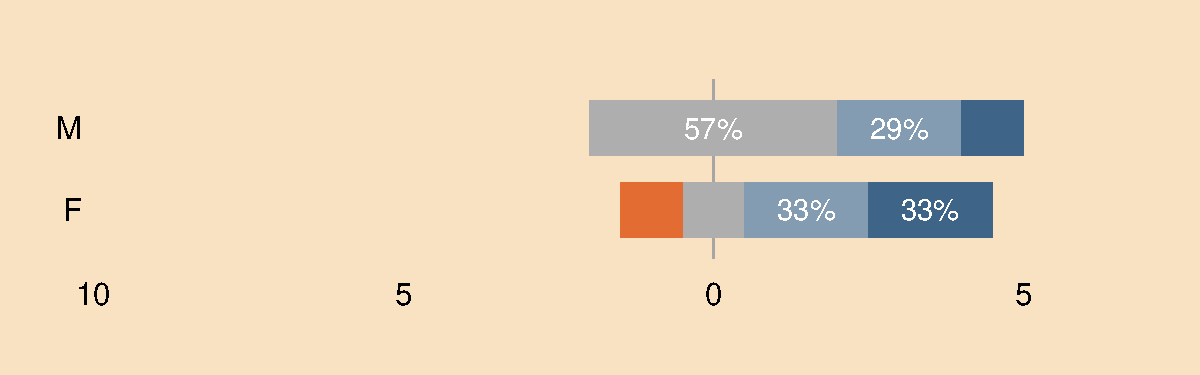
\includegraphics[align=t,trim={0mm 2mm 0 16mm},clip,width=10cm]{fig/support/dirk_supportV2eR.pdf}\\

    %% Legend
    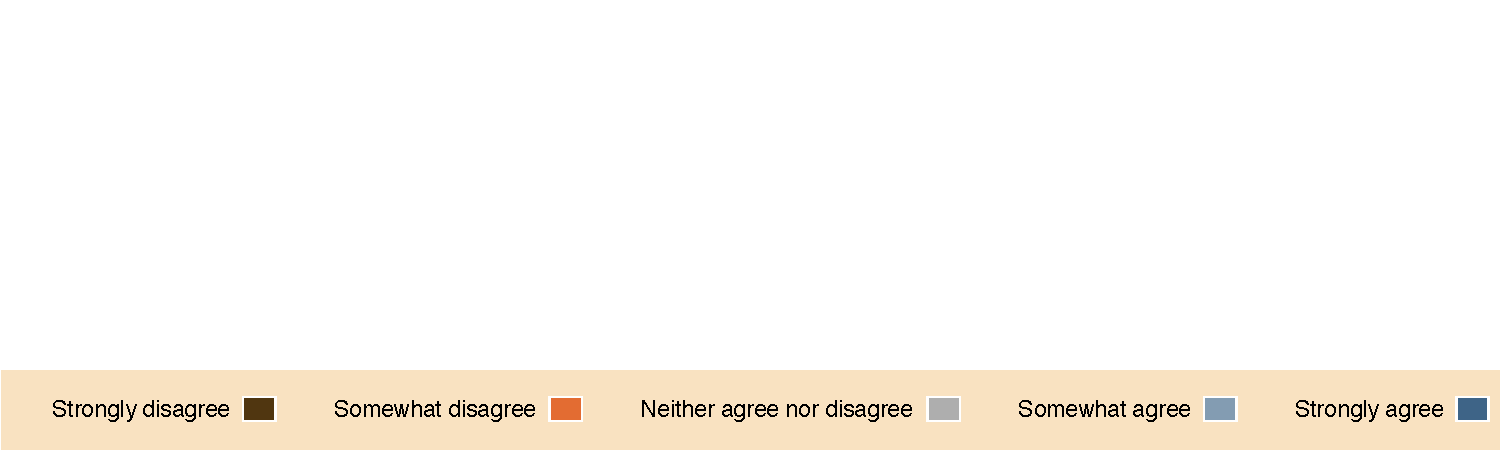
\includegraphics[trim={6mm 0 0 0},clip,width=14.5cm]{fig/legend5col.pdf}\\
    


\end{longfigure}
\end{mdframed}

%TC:endignore


While available opportunities to apply for funding were mostly satisfactory for both academics and researchers, a number of academics and researchers were dissatisfied. Further, most respondents also were satisfied with the support available within the school to apply for funding, a small number respondents were not. 
Less satisfied were a number of male academics with the support provided by the university, for example through the \ac{OVPRI} and the college. 
Finally, there is some room for improvement to provide support to those whose funding applications were not successful. While several respondents answered neutral (neither agree/disagree), male academics in particular found this lacking.








Success in attracting research funding is a key factor in academic career progression for both researchers and academics, and in response the school will create a programme to support staff before, during, and after the funding application process (Action~\ref{action:acad:supportfunding}). 


\begin{actionblock}{\ksspace{}Research funding support programme}{acad:supportfunding}
\actsupportprogramme
\hfill{
    \hypersetup{hidelinks}
    \hyperlink{c16}{\gotoactionsymbol{}}
}
\end{actionblock}



\subsubsection{Support for Development of Excellence in Teaching and Learning}

A qualification in teaching and learning is essential for promotion from Lecturer to Senior Lecturer so the school encourages all academic staff to avail of the courses offered by \ac{CIRTL}.

Academic survey respondents  were broadly satisfied with access to and support for equipment and digital tools, for teaching and research. The IT support group are held in high esteem. 

Research staff focus group respondents would like to have more clarity on opportunities to participate in tutoring, lecturing and other academic duties (Action~\ref{action:acad:handbook}).

\begin{actionblock}{\ksspace{}Opportunities for research staff to engage in school academic activities}{acad:handbook}
\acthandbook
\hfill{
    \hypersetup{hidelinks}
    \hyperlink{cxx1}{\gotoactionsymbol{}}
}
\end{actionblock}


\subsection{Comment and reflect on how workload is allocated and managed in the department (e.g. via a workload allocation model). This should include information on how the breadth of academic and research roles and responsibilities are captured in workload planning and allocation and results from staff consultation presented by gender.}\label{sub:workload}


\subsubsection{Workload Model and Allocation}

Academic staff workload includes teaching, research, and administration. Research staff primarily conduct research, but may also be asked to undertake light administrative tasks and/or contribute to teaching.
Research workload for academic staff is somewhat self-allocated and varies by staff member.
Workload is allocated by the \ac{HOS} 
to cover core teaching and administrative duties. 
New staff are assigned a reduced teaching load for their first year to enable them to develop their research agenda.
There is very limited recognition of research workload in the school's workload distribution scheme. This can result in a higher workload for research active staff. 

Workload allocation for research staff depends on their line manager and on their ambition.

\clearpage 

%TC:ignore

\begin{mdframed}[backgroundcolor=orangebg,
                 rightline=false,
                 leftline=false,
                 topline=false,
                 bottomline=false,
                 innertopmargin=0pt,
                 ]
\footnotesize                 
\begin{longfigure}{M{4.5cm}p{9.5cm}}
                    
               
\vspace*{-24pt}
\crule{12mm}{3mm}\\[-7mm]

\caption{Workload before and during Covid-19, by gender}
\label{fig:workload}\\


\endfirsthead
%
\endhead
%
\endfoot

\endlastfoot

\footnotesize

&\\

My workload is reasonable and balanced.   Academics, before Covid-19 &
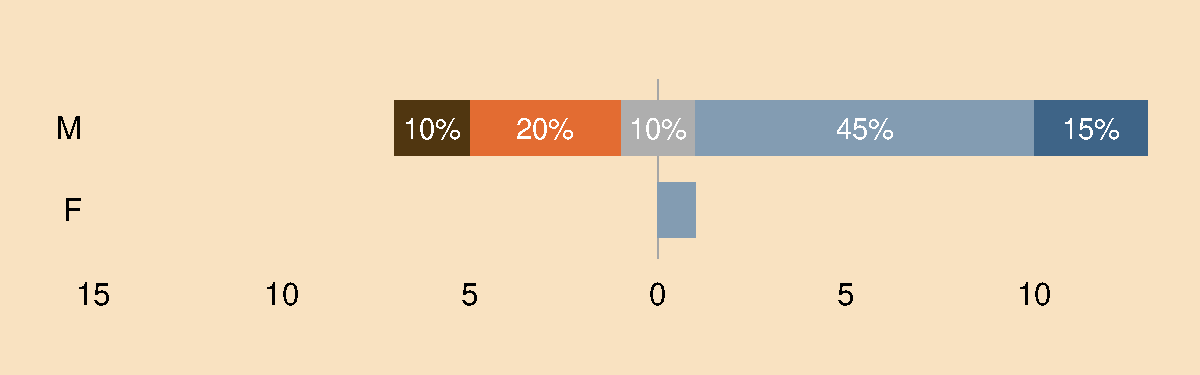
\includegraphics[align=t,trim={0mm 18mm 0 15mm},clip,width=10cm]{fig/workload/dirk_wload1A_pre}\\

Academics, during Covid-19 & 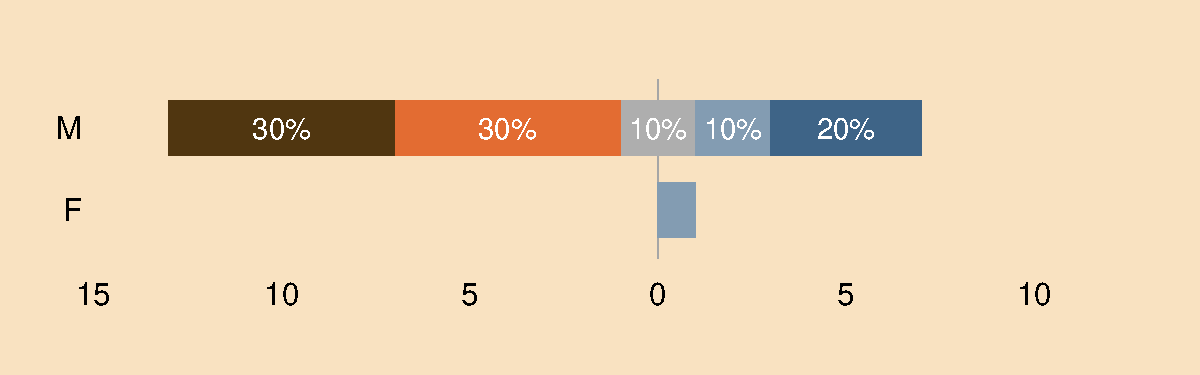
\includegraphics[align=t,trim={0mm 4mm 0 15mm},clip,width=10cm]{fig/workload/dirk_wload1A_during}\\

%My workload is reasonable and balanced.   
Researchers, before Covid-19 &
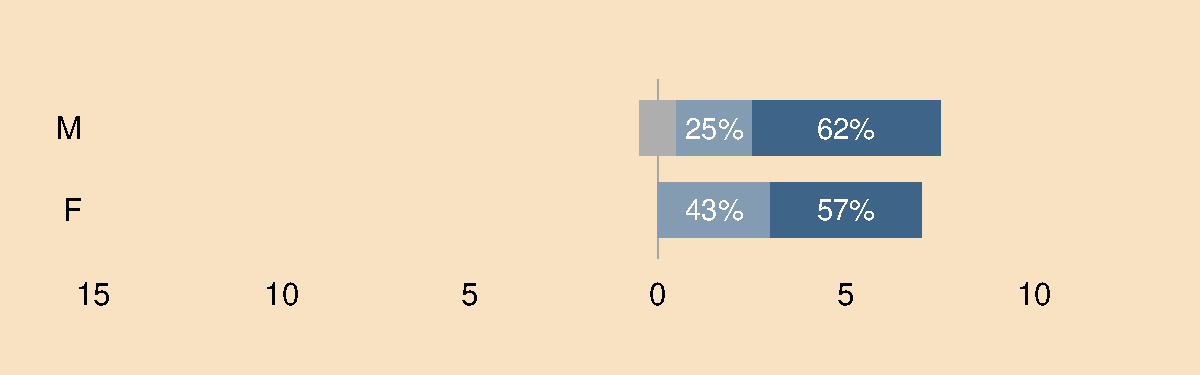
\includegraphics[align=m,trim={0mm 18mm 0 15mm},clip,width=10cm]{fig/workload/dirk_wload1R_pre}\\

Researchers, during Covid-19& 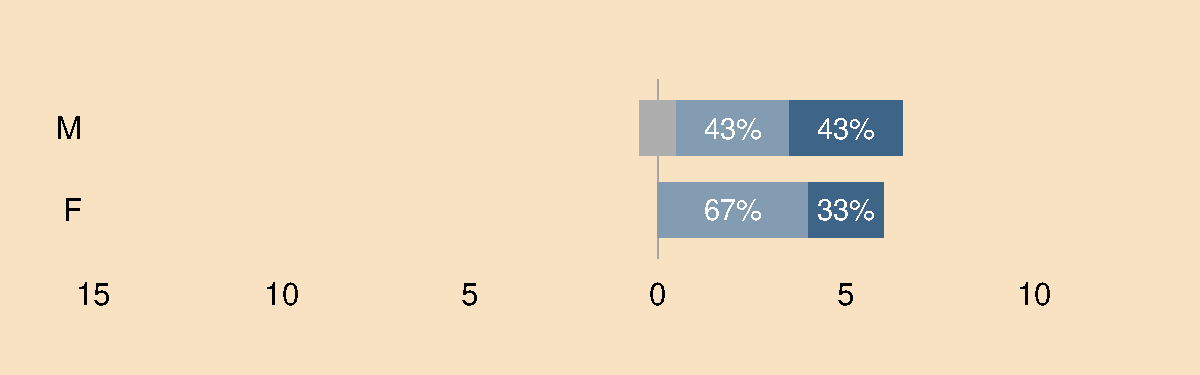
\includegraphics[align=t,trim={0mm 4mm 0 15mm},clip,width=10cm]{fig/workload/dirk_wload1R_during}\\


\hdashline

\addlinespace 
The school has a clear and transparent way of allocating workload.   Academics, before Covid-19  &
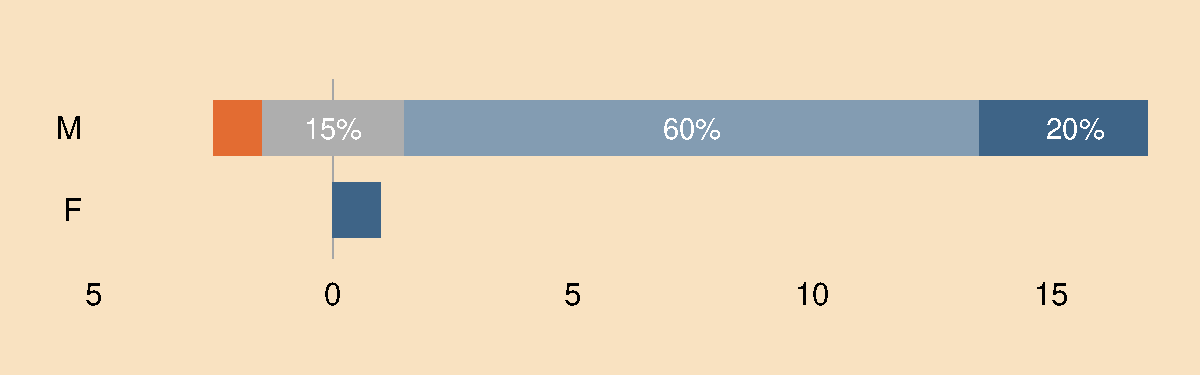
\includegraphics[align=m,trim={0mm 18mm 0 15mm},clip,width=10cm]{fig/workload/dirk_wload2A_pre}\\

Academics, during Covid-19  & 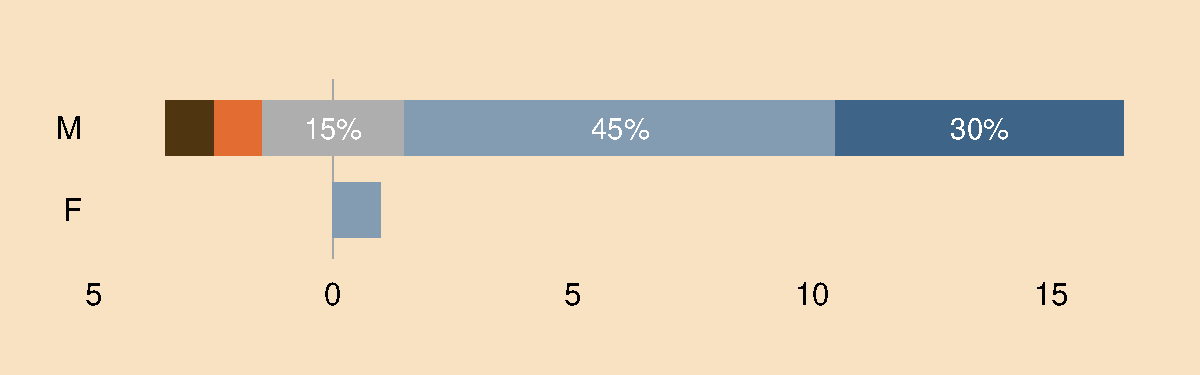
\includegraphics[align=m,trim={0mm 4mm 0 15mm},clip,width=10cm]{fig/workload/dirk_wload2A_during}\\


%The school has a clear and transparent way of allocating workload.   
Researchers, before Covid-19 &
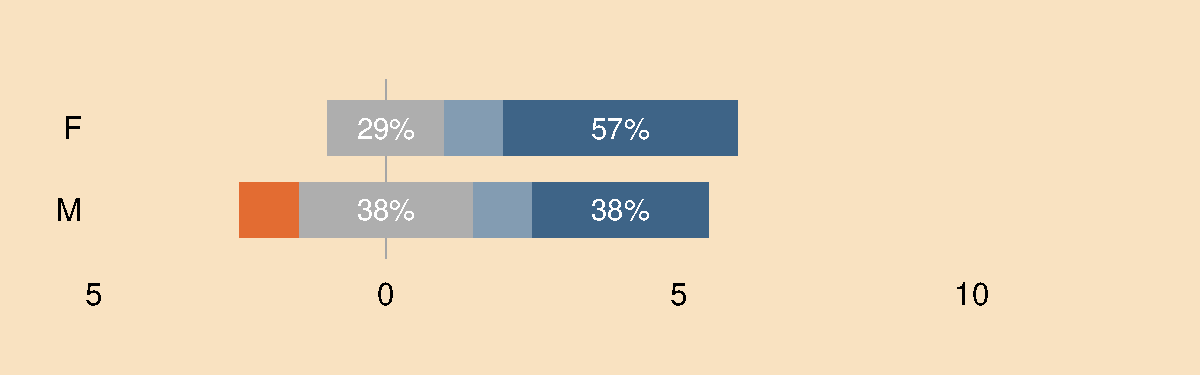
\includegraphics[align=m,trim={0mm 18mm 0 15mm},clip,width=10cm]{fig/workload/dirk_wload2R_pre}\\

Researchers, during Covid-19& 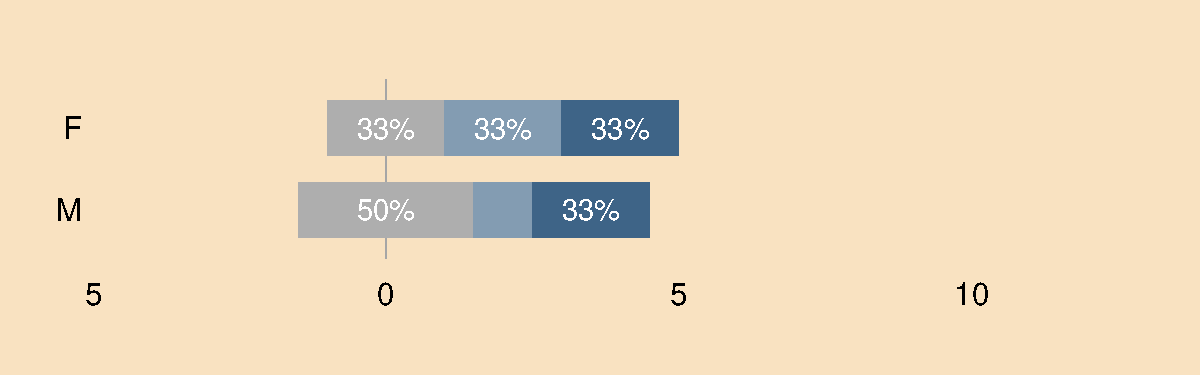
\includegraphics[align=m,trim={0mm 4mm 0 15mm},clip,width=10cm]{fig/workload/dirk_wload2R_during}\\

\hdashline
\pagebreak 
\multicolumn{2}{l}{\normalsize \textbf{Figure \thefigure{}} Workload before and during Covid-19, by  gender (continued)}\\
\addlinespace

The allocation of my workload aligns with my personal career development goals.   Academics, before Covid-19 &
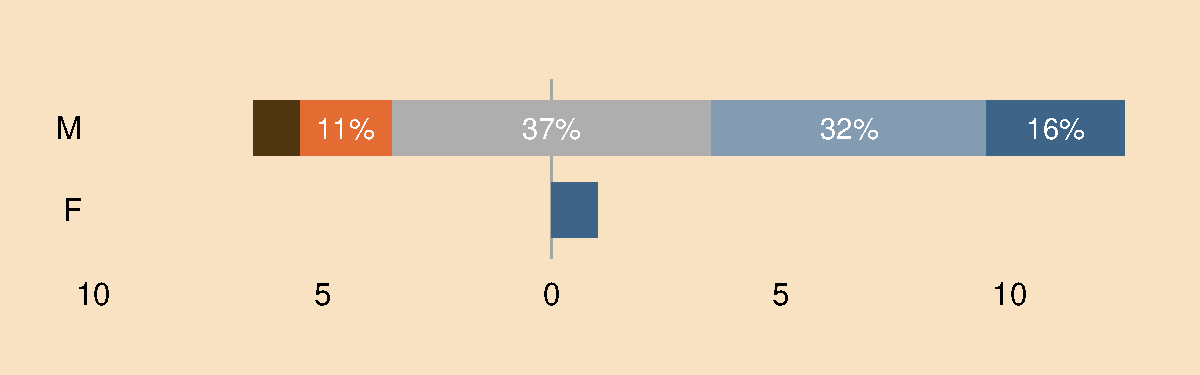
\includegraphics[align=t,trim={0mm 18mm 0 15mm},clip,width=10cm]{fig/workload/dirk_wload3A_pre}\\

Academics, during Covid-19  & 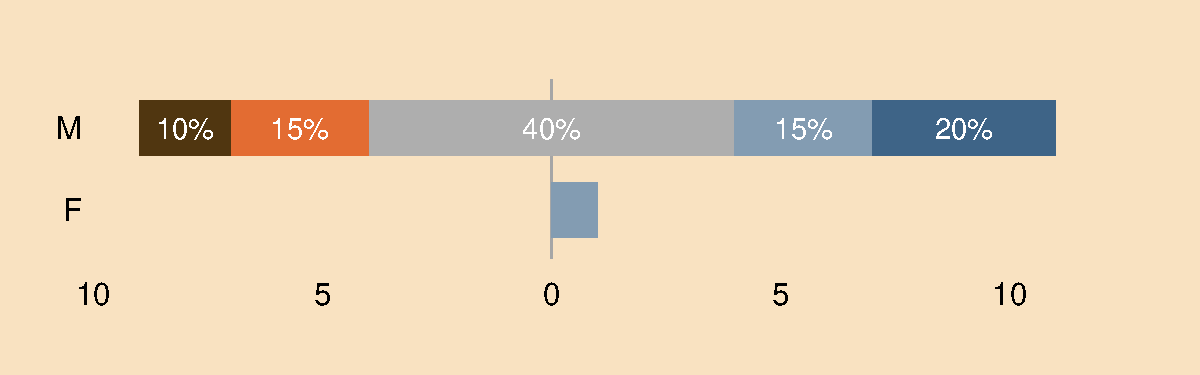
\includegraphics[align=m,trim={0mm 4mm 0 15mm},clip,width=10cm]{fig/workload/dirk_wload3A_during}\\


%The allocation of my workload aligns with my personal career development goals.  
Researchers, before Covid-19  &
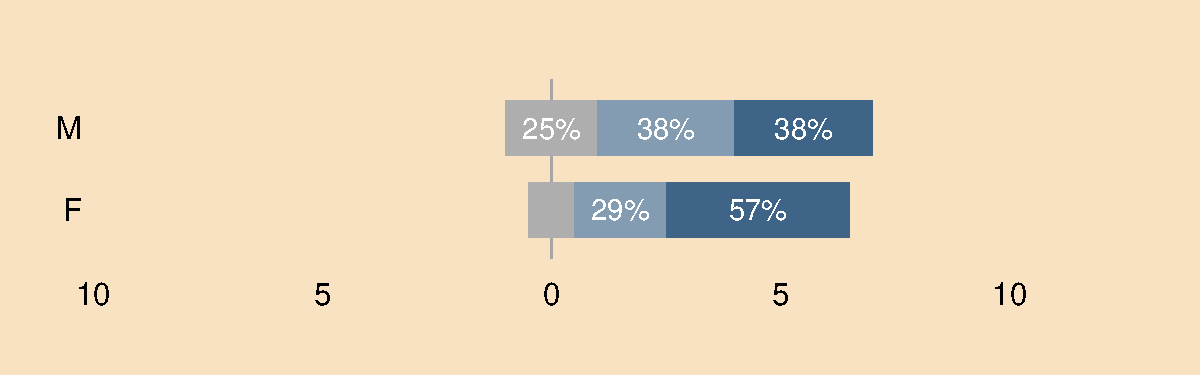
\includegraphics[align=m,trim={0mm 18mm 0 15mm},clip,width=10cm]{fig/workload/dirk_wload3R_pre}\\

Researchers, during Covid-19 & 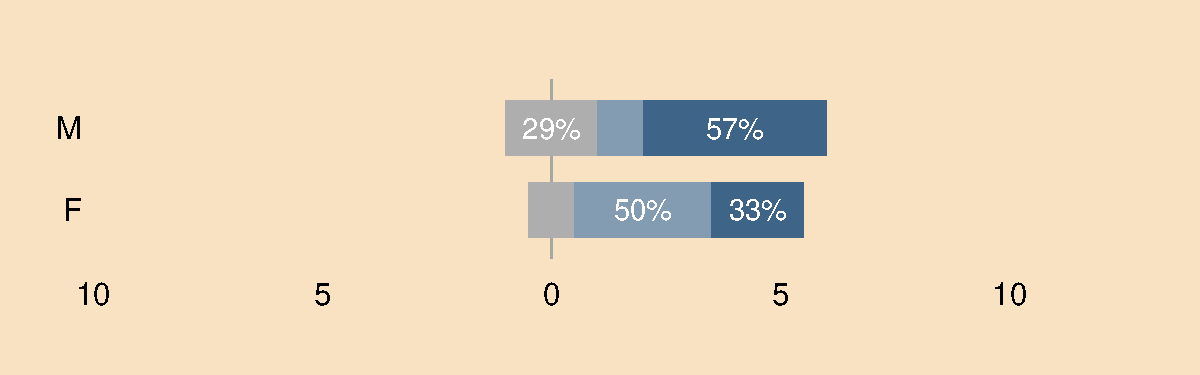
\includegraphics[align=m,trim={0mm 4mm 0 15mm},clip,width=10cm]{fig/workload/dirk_wload3R_during}\\

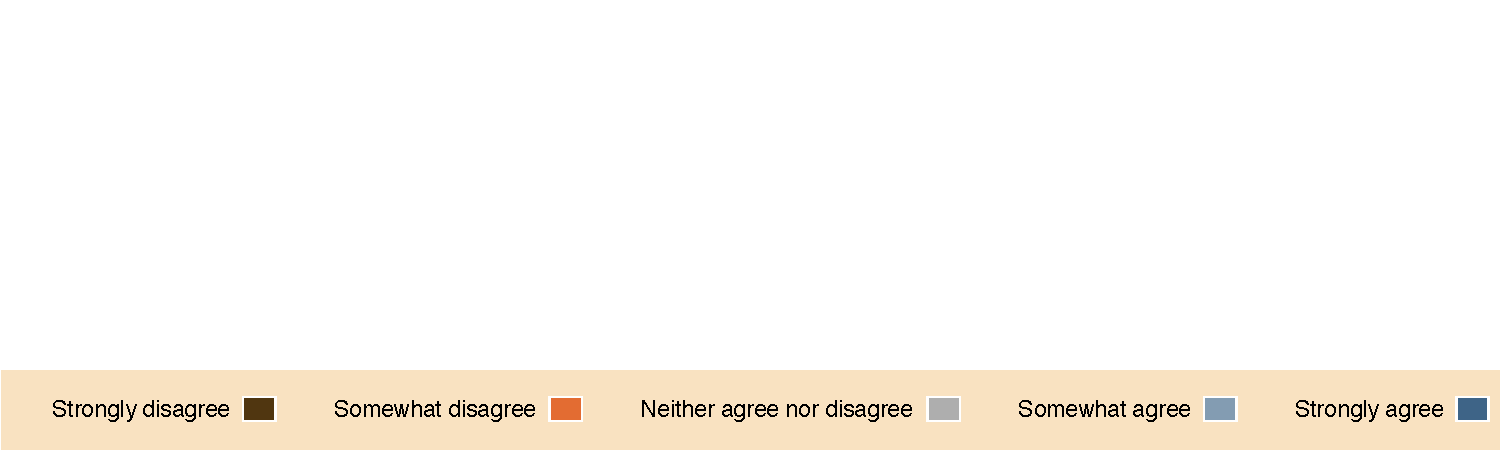
\includegraphics[trim={6mm 0 0 0},clip,width=14.5cm]{fig/legend5col.pdf}\\

\end{longfigure}
\end{mdframed}

%TC:endignore



\begin{figbox}{!t}
    \caption{Perceived changes to workload since Covid-19}
    % left lower right upper
    
    \label{fig:workloadchange}

    \sffamily
    \footnotesize
    \raggedright
    \begin{tabular}{P{3cm}
                    !{\qquad}
                    p{11cm}} 
    \addlinespace
    
    My workload has changed (Academics) &
    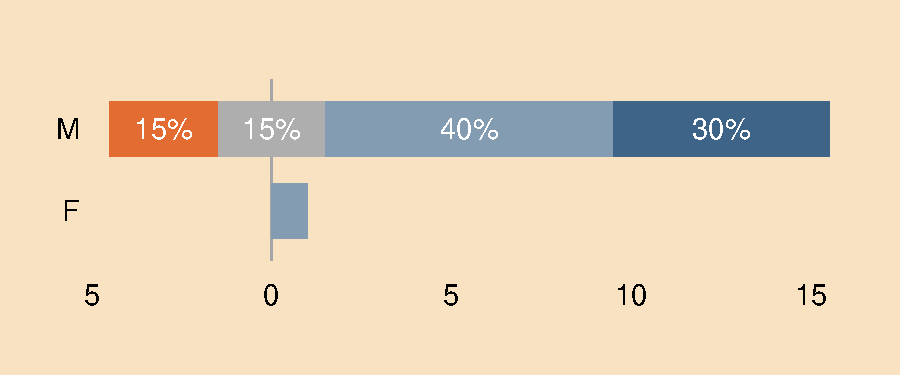
\includegraphics[align=t,trim={0mm 16mm 0 15mm},clip,width=8cm]{fig/workload/dirk_workload2aA.pdf}\\

    As above, for Researchers &
    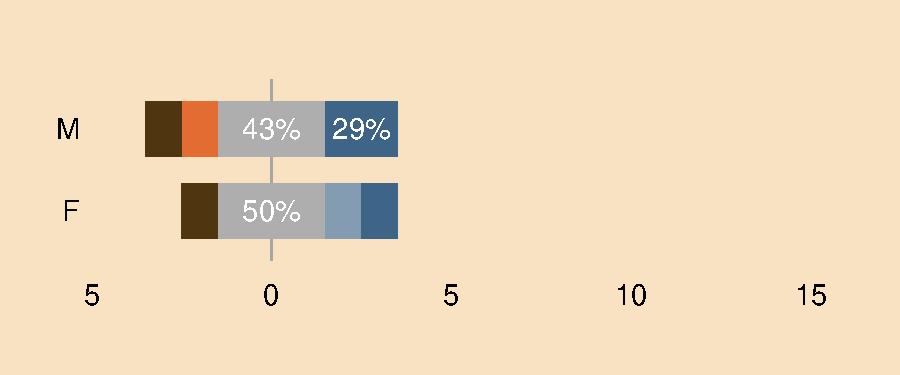
\includegraphics[align=t,trim={0mm 4mm 0 15mm},clip,width=8cm]{fig/workload/dirk_workload2aR.pdf}\\
    
    \hdashline
    
    Time spent completing my workload has changed (Academics) &
    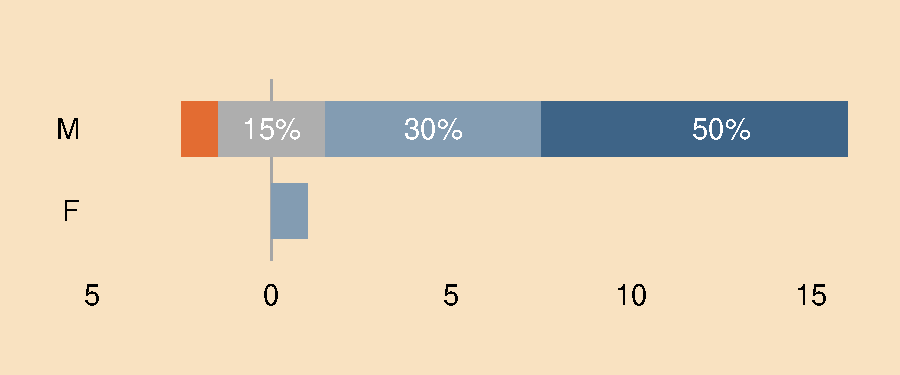
\includegraphics[align=t,trim={0mm 16mm 0 15mm},clip,width=8cm]{fig/workload/dirk_workload2bA.pdf}\\

    As above, for Researchers &
    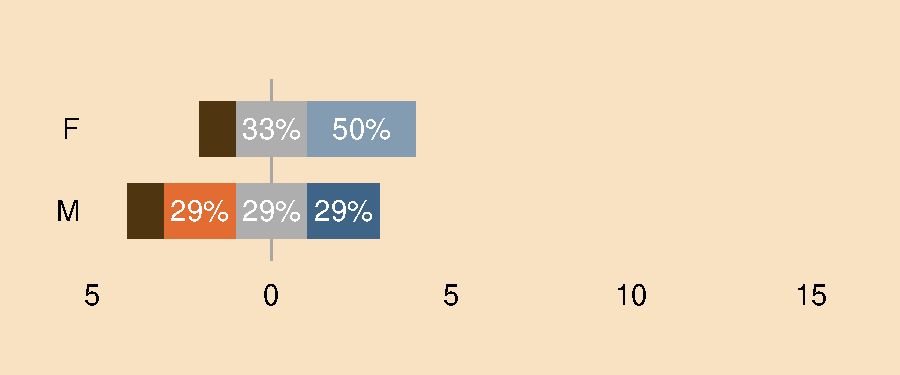
\includegraphics[align=t,trim={0mm 4mm 0 15mm},clip,width=8cm]{fig/workload/dirk_workload2bR.pdf}\\

    
    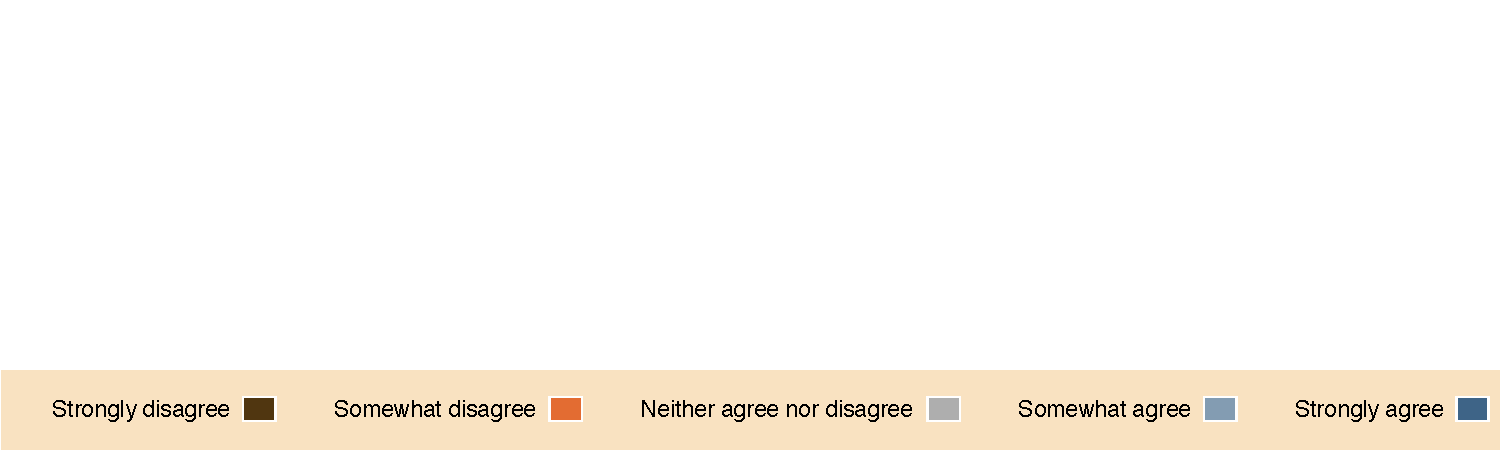
\includegraphics[trim={6mm 0 0 0},clip,width=14.5cm]{fig/legend5col.pdf}\\    
    \end{tabular}
\end{figbox}


The female academic felt that her workload was reasonable and balanced, that the scheme was transparent way, supporting her career goals. This did not change during the Covid-19 period (Figure~\ref{fig:workload} and Figure~\ref{fig:workloadchange}). 
Just over half of the male academics felt their workload allocation was reasonable and balanced; the majority felt that the allocation was clear and transparent. Only half said that the workload allocation aligned with their personal career development goals. Most male respondents felt that their workload was not balanced and had changed since the pandemic started. In the academic focus group, some colleagues commented on the ever-increasing number of administrative tasks, the scheduling of meetings, and the timing of tasks that may clash with caring responsibilities. 


\begin{myquote}
“Caring responsibilities are not considered when it comes to timing of meetings or academic responsibilities e.g. lecturing/labs. It is also not considered for workload.”
\end{myquote}

Both female and male  research staff respondents felt that their workload was reasonable and balanced (Figure~\ref{fig:workload}), whereas 50\% of female and male staff did not consider it to be clear and transparent. The majority of staff felt that their workload aligned with career development goals. However, problems remain:

\begin{myquote}
“If anything, the workload has increased considerably in the past 16 months [but] teamwork is good.”
\end{myquote}

In response, the school will review its workload model (Action~\ref{action:acad:transparentworkload}).


\begin{actionblock}{\ksspace{}Review workload model}{acad:transparentworkload}
\actreviewworkloadmodel
\hfill{
    \hypersetup{hidelinks}
    \hyperlink{c19}{\gotoactionsymbol{}}
}
\end{actionblock}




%% End of section.
